\def\tenchude{HỆ THỨC LƯỢNG TRONG TAM GIÁC}
\setcounter{section}{1}
\setcounter{dang}{0}
\section{HỆ THỨC LƯỢNG TRONG TAM GIÁC}
\subsection{Tóm tắt lý thuyết}
\subsubsection{Định lý cosin}
\immini{Cho tam giác $ ABC$ có $ BC=a$, $ AC=b$ và $ AB=c$.
	\begin{listEX}
		\item[$\bullet$] $ a^2=b^2+c^2-2bc\cdot \cos A \Rightarrow \cos A=$ \dotfill 
		\item[$\bullet$] $ b^2=c^2+a^2-2ca\cdot \cos B \Rightarrow \cos B=$ \dotfill 
		\item[$\bullet$] $ c^2=a^2+b^2-2ab\cdot \cos C \Rightarrow \cos A=$\dotfill 
	\end{listEX}
}
{\begin{tikzpicture}[scale=0.7,font=\footnotesize,line join=round, line cap=round,>=stealth]
		\tkzDefPoints{0/0/B,1/2/A,4/0/C}
		\tkzDrawPoints[fill=black](A,B,C)
		\tkzDefMidPoint(A,B) \tkzGetPoint{c}
		\tkzDefMidPoint(C,B) \tkzGetPoint{a}
		\tkzDefMidPoint(A,C) \tkzGetPoint{b}
		\tkzDrawPolygon(A,B,C)
		\tkzLabelPoints[above](A) 
		\tkzLabelPoints[below](B,C,a)
		\tkzLabelPoints[left](c)
		\tkzLabelPoints[right](b)
\end{tikzpicture}}
\subsubsection{Định lý sin}
\immini{
	Cho tam giác $ ABC$ có $ BC=a,AC=b$, $ AB=c$ và 
	$ R$ là bán kính đường tròn ngoại tiếp. 
	Ta có 
	$$ \dfrac{a}{\sin A}=\dfrac{b}{\sin B}=\dfrac{c}{\sin C}=2R$$
	\begin{note}
		Ghi nhớ: Tỉ lệ "cạnh chia sin góc đối" thì bằng nhau.
	\end{note}
}
{
	\begin{tikzpicture}[scale=0.6,font=\footnotesize,line join=round, line cap=round,>=stealth]
		\tkzDefPoints{0/0/B,1/3/A,4/0/C}
		\tkzCircumCenter(A,B,C) \tkzGetPoint{I}
		\tkzDrawPoints[fill=black](A,B,C,I)
		\tkzDrawCircle(I,A)
		\tkzDefMidPoint(A,B) \tkzGetPoint{c}
		\tkzDefMidPoint(C,B) \tkzGetPoint{a}
		\tkzDefMidPoint(A,C) \tkzGetPoint{b}
		\tkzDefMidPoint(a,c) \tkzGetPoint{R}
		\tkzDrawPolygon(A,B,C)
		\tkzDrawSegments(I,A I,B I,C)
		\tkzLabelPoints[above](A) 
		\tkzLabelPoints[below](B,C,a,I,R)
		\tkzLabelPoints[left](c)
		\tkzLabelPoints[right](b)
\end{tikzpicture}} 

\subsubsection{Công thức tính diện tích tam giác}
Gọi $S$ là diện tích tam giác $ABC$. Ta có
\begin{itemize}
	\item $S=\dfrac{1}{2}a\cdot h_a=\dfrac{1}{2}b\cdot h_b=\dfrac{1}{2}c\cdot h_c$,
	\item $S=\dfrac{1}{2}bc\sin A=\dfrac{1}{2}ca\sin B=\dfrac{1}{2}ab\sin C$,
	\item $S=\dfrac{abc}{4R}$, $S=p\cdot r$, (đọc thêm)
	\item $S=\sqrt{p(p-a)(p-b)(p-c)}$.
\end{itemize}
Trong đó:
\begin{itemize}
	\item [$\bullet$] $ h_a$, $h_b$, $h_c$ là độ dài đường cao lần lượt tương ứng với các cạnh $ BC$, $CA$, $AB$.
	\item [$\bullet$] $ R$ là bán kính đường tròn ngoại tiếp tam giác.
	\item [$\bullet$] $ r$ là bán kính đường tròn nội tiếp tam giác.
	\item [$\bullet$] $ p=\dfrac{a+b+c}{2}$ là nửa chu vi tam giác.
\end{itemize}

\subsection{Các dạng toán}
\begin{dang}{Áp dụng định lý cos}
	\textbf{Nhận dạng định lý:}
	\begin{itemize}
		\item [$\bullet$] Cho tam giác biết trước độ dài hai cạnh và số đo của một góc.
		\item [$\bullet$] Cho tam giác biết trước độ dài ba cạnh.
	\end{itemize}
\end{dang}
\viduminhhoa
\begin{vd}
	Cho tam giác $ABC$ có $b=5, c=7$ và $\cos A=\dfrac{3}{5}$. Tính cạnh $a$ và cosin các góc còn lại của tam giác đó.
	\loigiai{Ta có:
		\begin{align*}
			&a^2=b^2+c^2-2bc\cos A=25+49-2.5.7.\dfrac{3}{5}=32\Rightarrow a=\sqrt{32}=4\sqrt{2} \\
			&\cos B=\dfrac{c^2+a^2-b^2}{2ca}=\dfrac{32+49-25}{56\sqrt{2}}=\dfrac{\sqrt{2}}{2}\\
			&\cos C=\dfrac{a^2+b^2-c^2}{2ab}=\dfrac{32+25-49}{40\sqrt{2}}=\dfrac{8}{40\sqrt{2}}=\dfrac{\sqrt{2}}{10}.
		\end{align*}
	}
\end{vd}
\begin{vd}
	Cho tam giác $ABC$ có $AC = 10 \textrm{cm}, BC = 16 \textrm{cm}$ và $C=120^\circ$, tính độ dài cạnh $AB$.
	\loigiai{Áp dụng định lý hàm số cosin ta có $AB^2=CA^2+CB^2-2CA.CB\cos C$ ta suy ra $AB=\sqrt{516}\, \textrm{cm}$
	}
\end{vd}
\begin{note}
	Cho tam giác $ ABC$ có $ m_a$, $ m_b$, $ m_c$ lần lượt là các trung tuyến kẻ từ $ A$, $ B$, $ C$. 
	Ta có
	\immini{
		\begin{listEX}
			\item [$\bullet$] $ m_a^2=\dfrac{b^2+c^2}{2}-\dfrac{a^2}{4}$.
			\item [$\bullet$] $ m_b^2=\dfrac{a^2+c^2}{2}-\dfrac{b^2}{4}$.
			\item [$\bullet$] $ m_{c}^2=\dfrac{a^2+b^2}{2}-\dfrac{c^2}{4}$.
		\end{listEX}
	}
	{
		\begin{tikzpicture}[scale=0.7,font=\footnotesize,line join=round, line cap=round,>=stealth]
			\tkzDefPoints{0/0/B,1/3/A,6/0/C}
			\tkzDefMidPoint(A,B) \tkzGetPoint{c}
			\tkzDefMidPoint(C,B) \tkzGetPoint{a}
			\tkzDefMidPoint(A,C) \tkzGetPoint{b}
			\coordinate (m_a) at ($ (A)!0.4!(a)$ );
			\coordinate (m_b) at ($ (B)!0.4!(b)$ );
			\coordinate (m_c) at ($ (C)!0.4!(c)$ );
			\tkzDrawPoints[fill=black](A,B,C,a,b,c)
			\tkzDrawPolygon(A,B,C)
			\tkzDrawSegments(a,A b,B c,C)
			\tkzLabelPoints[above](A) 
			\tkzLabelPoints[below](B,C,a,m_b,m_c)
			\tkzLabelPoints[left](c,m_a)
			\tkzLabelPoints[above right](b)
	\end{tikzpicture}}
\end{note}
\begin{vd}
	Cho tam giác $ABC$ có $AB=4~\mathrm{cm}$, $AC=3 ~\mathrm{cm}$ và $BC=6 ~\mathrm{cm}$. Tính
	độ dài trung tuyến kẻ từ $C$ của tam giác $ABC$. 
	\loigiai{	\immini{Độ dài trung tuyến kẻ từ $C$ của tam giác $ABC$ là
			\\
			$ m_{c}^2=\dfrac{a^2+b^2}{2}-\dfrac{c^2}{4}= \dfrac{6^2 + 3^2}{2} - \dfrac{4^2}{4} =\dfrac{37}{2} \Rightarrow m_c = \dfrac{\sqrt{74}}{2}$.	
		}
		{
			\begin{tikzpicture}[scale=0.7,font=\footnotesize,line join=round, line cap=round,>=stealth]
				\tkzDefPoints{0/0/B,1/3/A,6/0/C}
				\tkzDefMidPoint(A,B) \tkzGetPoint{c}
				\tkzDefMidPoint(C,B) \tkzGetPoint{a}
				\tkzDefMidPoint(A,C) \tkzGetPoint{b}
				\coordinate (m_a) at ($ (A)!0.3!(a)$ );
				\coordinate (m_b) at ($ (B)!0.3!(b)$ );
				\coordinate (m_c) at ($ (C)!0.3!(c)$ );
				\tkzDrawPoints[fill=black](A,B,C,a,b,c)
				\tkzDrawPolygon(A,B,C)
				\tkzDrawSegments(a,A b,B c,C)
				\tkzLabelPoints[above](A) 
				\tkzLabelPoints[below](B,C,a,m_b,m_c)
				\tkzLabelPoints[left](c,m_a)
				\tkzLabelPoints[above right](b)
\end{tikzpicture}}}\end{vd}
\begin{vd}
	Cho tam giác $ABC$ có $BC=3, CA=4$ và $AB=6$. Tính cosin của góc có số đo lớn nhất của tam giác đã cho.
	\loigiai{Do $AB>AC>BC$ nên $C>B>A$.\\
		Áp dụng định lý hàm số cosin ta có $\cos C=-\dfrac{11}{24}.$
	}
\end{vd}
\begin{vd}
	\immini
	{
		Hai chiếc tàu thủy cùng xuất phát từ một vị trí $ A$, đi thẳng theo hai hướng tạo với nhau góc $ 60^\circ$. Tàu $ B$ chạy với tốc độ $ 20$ hải lí một giờ. Tàu $ C$ chạy với tốc độ $ 15$ hải lí một giờ. Hỏi sau hai giờ, hai tàu cách nhau bao nhiêu hải lí?
	}
	{
		\begin{tikzpicture}[line join=round, line cap=round,>=stealth,scale=1]
			\foreach \x in {1,2,3}
			\foreach \y in {0,1,2,3,4,5}
			\draw(0.25+\y,\x-0.25)--(\y,\x-0.25) ;
			\foreach \x in {1,2,3}
			\foreach \y in {0,1,2,3,4,5}
			\draw(-0.25+\y,\x-0.75)--(\y,\x-0.75) ;
			\tkzDefPoints{0/0/A,4/0/B,1.5/2.5/C}
			\tkzDefMidPoint(A,B) \tkzGetPoint{40}
			\tkzDefMidPoint(A,C) \tkzGetPoint{30} 
			\tkzDrawPoints[fill=black](A,B,C)
			\tkzDrawSegments(A,B A,C)
			\fill plot [smooth cycle] coordinates{(3.75,0)(4.25,0)(4.3,0.2)(4.15,0.2)(4.15,0.3)(4.05,0.3)(4.05,0.4)(3.95,0.4)(3.95,0.3)(3.85,0.3)(3.85,0.2)(3.7,0.2)} ;
			\fill plot [smooth cycle] coordinates{(1.25,2.5)(1.75,2.5)(1.8,2.7)(1.65,2.7)(1.65,2.8)(1.55,2.8)(1.55,2.9)(1.45,2.9)(1.45,2.8)(1.35,2.8)(1.35,2.7)(1.2,2.7)} ;
			\tkzLabelPoints[below](A,B,C,40)
			\tkzLabelPoints[left](30)
		\end{tikzpicture}
	}
	\loigiai{
		Sau $ 2$ giờ tàu $ B$ đi được $ 40$ hải lí, tàu $ C$ đi được $ 30$ hải lí. \\
		Vậy tam giác $ ABC$ có $ AB=40$, $AC=30$ và $ \widehat{A}=60^\circ$. \\
		Áp dụng định lí cosine vào tam giác $ ABC$, ta có
		$$ a^2=b^2+c^2-2bc\cdot\cos A=30^2+40^2-2\cdot 30\cdot 40\cdot \cos 60^\circ=1300\Rightarrow a\simeq 36.$$ 
		Vậy sau $ 2$ giờ, hai tàu cách nhau khoảng $ 36$ hải lí.}
\end{vd}
\begin{vd}%[0H2B3-2]
	Tam giác $ABC$ có $AB= c$; $BC=a$; $CA= b.$ Các cạnh $a$, $b$, $c$ liên hệ với nhau bởi đẳng thức $b(b^2 -a^2) = c(a^2 -c^2)$. Tính số đo góc $\widehat{BAC}$.
	\loigiai{
		Theo định lý hàm côsin, ta có $$\cos \widehat{BAC}= \dfrac{AB^2 + AC^2 - BC^2}{2 \cdot AB\cdot AC}= \dfrac{c^2 + b^2 -a^2}{2bc}.$$
		Mà 
		\begin{eqnarray*}
			& & b(b^2 -a^2) = c(a^2 -c^2) \\ 
			& \Leftrightarrow & b^3 -a^2 b = a^2 c -c^3 \\
			& \Leftrightarrow &-a^2 (b+c) + (b+c)(b^2 + c^2 -bc)=0\\
			& \Leftrightarrow & b^2 + c^2 - a^2 =bc.
		\end{eqnarray*} 
		Khi đó $\cos \widehat{BAC} = \dfrac{bc}{2bc}= \dfrac{1}{2}$.\\
		Vậy $\widehat{BAC}= 60^\circ$.
	}
\end{vd}
\baitaptl
\begin{bt}
	Cho tam giác $ABC$ có $\widehat{A} = 60^\circ$, $AB=6$, $AC=8$. Tính $BC$.
	\loigiai{Áp dụng định lý cosine trong tam giác $ABC$ ta có $BC^2=AB^2 +AC^2 -2AB\cdot AC \cdot \cos A=6^2 +8^2 -2\cdot6\cdot 8 \cos 60^\circ = 52 \Rightarrow BC=2\sqrt{13}$.}
\end{bt}
\begin{bt}
	Cho tam giác $ABC$ có các cạnh $BC=6$, $CA=4\sqrt{2}$, $AB=2$. Tính $\cos A$ và góc $\widehat{A}$.
	\loigiai{Áp dụng hệ quả của định lý cosine ta có\\
		$\cos A = \dfrac{AB^2+AC^2 -BC^2}{2AB \cdot AC}= \dfrac{2^2 + \left(4\sqrt{2}\right)^2 -6^2}{2\cdot 2\cdot 4\sqrt{2}} =0 \Leftrightarrow \widehat{A}=90^\circ $.}
\end{bt}
\begin{bt}
	Cho tam giác $ABC$ có $AB=6$ cm; $AC =5$ cm và $\widehat{ACB}=60^\circ$. Tính $BC$.
	\loigiai{ Áp dụng định lý cosine trong tam giác ta có\\ $AB^2 =AC^2 +BC^2 -2AC\cdot BC \cdot \cos \widehat{ACB}$ $\Rightarrow 6^2 =5^2 +BC^2 -2\cdot 5 \cdot BC \cos 60^\circ$\\ $\Leftrightarrow BC^2 -5BC-11=0 \Leftrightarrow BC =\dfrac{5+ \sqrt{69}}{2}$.}
\end{bt}
\begin{bt}
	Tam giác $ABC$ có $b= 6$, $c= 8$ và $m_a= 5$. Tính $a$, $\widehat{A}$.
	\loigiai{Áp dụng công thức đường trung tuyến trong tam giác ta có 
		\\
		$m_a^2 = \dfrac{b^2+c^2}{2} -\dfrac{a^2}{4} \Leftrightarrow 5^2 = \dfrac{6^2+8^2}{2} - \dfrac{a^2}{4} \Leftrightarrow a=10$.
	}
\end{bt}
\begin{bt}%[0H2K3]
	Cho tam giác $ABC$, gọi $l_a$ là độ dài đường phân giác trong kẻ từ đỉnh $A$ của tam giác $ABC$. Chứng minh rằng $l_a=\dfrac{bc\sin A}{(b+c)\sin\frac{A}{2}}$.
	\loigiai{
		\immini{
			Gọi $D$ là chân đường phân giác trong kẻ từ đỉnh $A$ của tam giác $ABC$. Ta có $l_a=AD$. Ta có
			$$\begin{aligned}
				&S_{ABC}=S_{ABD}+S_{ACD}\\
				\Leftrightarrow &\dfrac{1}{2}AB.AC.\sin A=\dfrac{1}{2}AB.AD.\sin \frac{A}{2}+\dfrac{1}{2}AC.AD.\sin \frac{A}{2}\\
				\Leftrightarrow & cb\sin A=l_a(c+b)\sin\frac{A}{2}\\
				\Leftrightarrow &l_a=\dfrac{bc\sin A}{(b+c)\sin\frac{A}{2}}
			\end{aligned}$$
		}{
			% \begin{tikzpicture}
			% 	\clip (-3,-3) rectangle (4,2);
			% 	\tkzDefPoints{0/1/A,-1/-2/B,3/-2/C}
			% 	\draw (A)node[above]{$A$}--(B)node[below]{$B$}--(C)node[below]{$C$}--(A);
			% 	\tkzInCenter(A,B,C) \tkzGetPoint{I}
			% 	\tkzInterLL(B,C)(A,I) \tkzGetPoint{D}
			% 	\tkzDrawBisector(B,A,C)
			% 	\tkzLabelPoints[below](D)
			% 	\tkzMarkAngle[size=0.5](D,A,C)
			% 	\tkzMarkAngle[size=0.6](B,A,D)
			% \end{tikzpicture}
		}
	}
\end{bt}
\begin{bt}
	Hai lực $\overrightarrow{f_1}$ và $\overrightarrow{f_2}$ cho trước cùng tác dụng lên một vật và tạo thành góc nhọn $\left(\overrightarrow{f_1},\overrightarrow{f_2}\right)=\alpha$. Hãy lập công thức tính cường độ của hợp lực $\overrightarrow{s}$.
	\loigiai{
		\centerline{
			\begin{tikzpicture}[>=stealth,scale=1]
				\tkzDefPoints{0/0/A,1/2/B}
				\tkzDefShiftPoint[A](0:4){D}
				\tkzDefShiftPoint[B](0:4){C}
				\tkzDrawSegments[->](A,B A,D A,C)
				\tkzDrawSegments(B,C C,D)
				\tkzLabelPoints[left](B,A)
				\tkzLabelPoints[right](C,D)
				\tkzMarkAngles[mkpos=.2,size=.3](D,A,B A,B,C)
				\tkzLabelAngle[pos=.6](D,A,B){\footnotesize $\alpha$}
				\tkzLabelLine[pos=.5,left](A,B){\footnotesize $\overrightarrow{f_1}$}
				\tkzLabelLine[pos=.5,below](A,D){\footnotesize $\overrightarrow{f_2}$}
				\tkzLabelLine[pos=.5,above left](A,C){\footnotesize $\overrightarrow{s}$}
		\end{tikzpicture}}\\
		Đặt $\overrightarrow{AB}=\overrightarrow{f_1}, \overrightarrow{AD}=\overrightarrow{f_2}$ và vẽ hình bình hành $ABCD$.\\
		Khi đó $\overrightarrow{AC}=\overrightarrow{AB}+\overrightarrow{AD}=\overrightarrow{f_1}+\overrightarrow{f_2}=\overrightarrow{s}$.\\
		Vậy $\left|\overrightarrow{s}\right|=\left|\overrightarrow{AC}\right|=\left|\overrightarrow{f_1}+\overrightarrow{f_2}\right|$.\\
		Theo định lí côsin đối với tam giác $ABC$, ta có:\\
		$AC^2=AB^2+BC^2-2.AB.BC.\cos B$, hay $\left|\overrightarrow{s}\right|^2=\left|\overrightarrow{f_1}\right|^2+\left|\overrightarrow{f_2}\right|^2-2\left|\overrightarrow{f_1}\right|.\left|\overrightarrow{f_2}\right|.\cos(180^\circ-\alpha)$.\\
		Do đó: $\left|\overrightarrow{s}\right|=\sqrt{\left|\overrightarrow{f_1}\right|^2+\left|\overrightarrow{f_2}\right|^2+2\left|\overrightarrow{f_1}\right|.\left|\overrightarrow{f_2}\right|.\cos\alpha}$.
	}
\end{bt}
\begin{dang}{Áp dụng định lý sin}
\textbf{Nhận dạng định lý:}
\begin{itemize}
	\item [$\bullet$] Cho tam giác biết trước độ dài hai cạnh và số đo của một góc.
	\item [$\bullet$] Cho tam giác biết trước độ dài một cạnh và số đo của hai góc.
	\item [$\bullet$] Cho tam giác biết trước độ dài một cạnh, số đo góc đối diện và bán kính đường tròn ngoại tiếp tam giác.
\end{itemize}
\end{dang}
\viduminhhoa
\begin{vd}%[Phạm Tuấn]%[0H2B3-1] 
	Cho tam giác $ABC$ có $\widehat{A}= 120^\circ$ và $BC= 10 \mathrm{~cm}$. Tính bán kính đường tròn ngoại tiếp tam giác $ABC$.
	\loigiai{
		Áp dụng định lí sin ta có $R = \dfrac{BC}{2\sin A} = \dfrac{10}{2\sin 120^\circ} = \dfrac{10\sqrt{3}}{3} \mathrm{~cm}$. 
	}
\end{vd}


\begin{vd}%[Phạm Tuấn]%[0H2B3-1] 
	\immini{
		Cho tam giác $ABC$ có $\widehat{A}= 40^\circ$, $\widehat{B}=55^\circ$ và $AB = 100$. Tính độ dài cạnh $BC$ (làm tròn kết quả đến hàng phần mười).
	}
	{
		\begin{tikzpicture}[scale=1, font=\footnotesize, line join=round, line cap=round,>=stealth]
			\path
			(0,0) coordinate (A)
			(4,0) coordinate (B)
			;
			\coordinate (A') at ($(A)+(40:3)$); 
			\coordinate (B') at ($(B)+(-55:3)$); 
			\coordinate (C) at (intersection of A--A' and B--B');
			\draw (A)--(B)--(C)--(A);
			
			\tkzMarkAngle[arc=ll,size=0.5,mark=0](B,A,C)
			\tkzLabelAngle[pos=1.1](B,A,C) {$40^\circ$}
			\tkzMarkAngle[arc=l,size=0.5,mark=0](C,B,A)
			\tkzLabelAngle[pos=0.8](C,B,A) {$55^\circ$}
			\foreach \x/\g in {A/-120,B/-60,C/90} 
			\fill[black] (\x) circle (1pt)+(\g:3mm) node {$\x$};
		\end{tikzpicture}
	}
	\loigiai{
		Ta có $\widehat{C}= 180^\circ -  \widehat{A} -\widehat{B} = 180^\circ - 40^\circ-55^\circ  =85^\circ$. \\
		Áp dụng định lí sin ta có 
		\[
		\dfrac{AB}{\sin C} = \dfrac{BC}{\sin A} \Rightarrow BC = \dfrac{AB\sin A}{\sin C}  = \dfrac{100\sin 40^{\circ}}{\sin 85^{\circ}} \approx 64{,}5. 
		\]
	}
\end{vd}


\begin{vd}%[Phạm Tuấn]%[0H2B3-1] 
	Cho tam giác $ABC$ có $\dfrac{AB}{2} = \dfrac{BC}{3}$ và $\widehat{A} = 45^\circ$. Tính các góc $B$, $C$  của tam giác đó (làm tròn kết quả đến hàng phần mười).
	\loigiai{
		Áp dụng định lí sin ta có
		\[
		\dfrac{AB}{\sin C}  = \dfrac{BC}{\sin A} \Rightarrow \sin C = \dfrac{AB\sin A}{BC} = \dfrac{2\sin 45^\circ}{3} \Rightarrow \widehat{C} \approx 
		28{,}1^\circ.\]
		Khi đó $\widehat{B}= 180^\circ - \widehat{A}- \widehat{C}= 180^\circ - 45^\circ -28{,}1^\circ=106{,}9^\circ $.
	}
\end{vd}


\begin{vd}%[Phạm Tuấn]%[0H2B3-1] 
	Cho tam giác $ABC$ có $\widehat{A}= 30^\circ$, $\widehat{B}=50^\circ$ và bán kính đường tròn ngoại tiếp bằng $10 \mathrm{~cm}$. Tính độ dài các cạnh của tam giác $ABC$ (làm tròn đến hàng phần mười).
	\loigiai{
		Ta có $\widehat{C}= 180^\circ - \widehat{A} - \widehat{B} =  180^\circ  -30^\circ - 50^\circ= 100^\circ$.  \\
		Áp dụng định lí sin
		\begin{align*}
			&  AB = 2R\sin C = 2\cdot 10 \cdot \sin 100^\circ \approx 19{,}7 \mathrm{~cm}; \\
			& BC = 2R\sin A = 2\cdot 10 \cdot \sin 30^\circ  = 10 \mathrm{~cm};  \\
			&AC = 2R\sin B = 2\cdot 10 \cdot \sin 50^\circ \approx 15{,}3 \mathrm{~cm}.
		\end{align*}
	}
\end{vd}


\begin{vd}%[Phạm Tuấn]%[0H2B3-1] 
	Cho tam giác $ABC$. Chứng minh rằng  $\sin^2 A = \sin B \sin C$ khi và chỉ khi $a^2 = bc$. 
	\loigiai{
		Theo định lí sin ta có  $\sin A = \dfrac{a}{2R}$;   $\sin B = \dfrac{b}{2R} $; $\sin C = \dfrac{c}{2R}$. \\
		Do đó 
		\[
		\sin^2 A = \sin B \sin C  \Leftrightarrow \left (\dfrac{a}{2R}\right )^2 =  \dfrac{b}{2R} \cdot  \dfrac{c}{2R} \Leftrightarrow a^2 = bc. 
		\]
	}
\end{vd}

\begin{vd}%[Phạm Tuấn]%[0H2B3-1] 
	Cho tam giác $ABC$.  Biết $AB= 5 \mathrm{~cm}$,  $BC= 6 \mathrm{~cm}$ và $2\sin A = \sin B + \sin C$. Tính độ dài cạnh $AC$. 
	\loigiai{
		Theo định lí sin ta có  $\sin A = \dfrac{BC}{2R}$;   $\sin B = \dfrac{AC}{2R} $; $\sin C = \dfrac{AB}{2R}$. \\
		Do đó 
		\[
		2\sin  A = \sin B +  \sin C  \Leftrightarrow \dfrac{2BC}{2R} =  \dfrac{AC}{2R} +  \dfrac{AB}{2R} \Leftrightarrow 2BC =AC+AB. 
		\]
		Suy ra $AC= 2BC-AB=  12 -5 =7    \mathrm{~cm}$. 
	}
\end{vd}

\baitaptl

\begin{bt}%[Phạm Tuấn]%[0H2B3-1] 
	Cho tam giác $ABC$ có $\widehat{B}= 70^\circ$ và $AC= 15 \mathrm{~cm}$. Tính bán kính đường tròn ngoại tiếp tam giác $ABC$ (làm tròn kết quả đến hàng phần mười).
	\loigiai{
		Áp dụng định lí sin ta có $R = \dfrac{AC}{2\sin B} = \dfrac{15}{2\sin 70^\circ} \approx 8 \mathrm{~cm}$. 
	}
\end{bt}


\begin{bt}%[Phạm Tuấn]%[0H2B3-1] 
	Cho tam giác $ABC$ có $\widehat{B}= 30^\circ$, $\widehat{C}=65^\circ$ và $BC = 50$. Tính độ dài cạnh $AB$ (làm tròn kết quả đến hàng phần mười).
	\loigiai{
		Ta có $\widehat{A}= 180^\circ -  \widehat{B} -\widehat{C} = 180^\circ - 30^\circ-65^\circ  =75^\circ$. \\
		Áp dụng định lí sin ta có 
		\[
		\dfrac{AB}{\sin C} = \dfrac{BC}{\sin A} \Rightarrow AB = \dfrac{BC\sin C}{\sin A}  = \dfrac{50\sin 65^{\circ}}{\sin 75^{\circ}} \approx 46{,}9. 
		\]
	}
\end{bt}

\begin{bt}%[Phạm Tuấn]%[0H2B3-1] 
	Cho tam giác $ABC$ có $\dfrac{BC}{3} = \dfrac{AC}{5}$ và $\widehat{A} = 30^\circ$. Tính các góc $B$, $C$  của tam giác đó (làm tròn kết quả đến hàng phần mười).
	\loigiai{
		Áp dụng định lí sin ta có
		\[
		\dfrac{AC}{\sin B}  = \dfrac{BC}{\sin A} \Rightarrow \sin B = \dfrac{AC\sin A}{BC} = \dfrac{5\sin 30^\circ}{3} \Rightarrow B \approx 
		56{,}4^\circ.\]
		Khi đó $\widehat{C}= 180^\circ - \widehat{A}- \widehat{B}= 180^\circ - 30^\circ -56{,}4^\circ=93{,}6^\circ $.
	}
\end{bt}

\begin{bt}%[Phạm Tuấn]%[0H2B3-2] 
	Cho tam giác $ABC$ thỏa mãn $a \sin B = c \sin A$.  Chứng minh rằng tam giác $ABC$ cân.
	\loigiai{
		Từ giả thiết suy ra $\dfrac{a}{\sin A} = \dfrac{c}{\sin B}$.  \quad (1)\\
		Áp dụng định lí sin ta có  $\dfrac{a}{\sin A} = \dfrac{b}{\sin B}$. \quad (2) \\
		Từ (1) và (2) suy ra $\dfrac{c}{\sin B} = \dfrac{b}{\sin B} \Rightarrow b=c$. \\
		Vậy tam giác $ABC$ cân. 
	}
\end{bt}

\begin{bt}%[Phạm Tuấn]%[0H2B3-2] 
	Cho tam giác $ABC$ thỏa mãn $\sin^2A = \sin^2B + \sin^2 C$.  Chứng minh rằng tam giác $ABC$ vuông. 
	\loigiai{
		Từ định lí sin suy ra $\sin A = \dfrac{a}{2R}$, $\sin B = \dfrac{b}{2R}$, $\sin C = \dfrac{c}{2R}$. \\
		Khi đó 
		\[
		\sin^2A = \sin^2B + \sin^2 C \Leftrightarrow \left (\dfrac{a}{2R}\right )^2 = \left (\dfrac{b}{2R}\right )^2 +\left (\dfrac{c}{2R}\right )^2 \Leftrightarrow a^2=b^2+c^2.
		\]
		Vậy tam giác $ABC$ vuông tại $A$. 
	}
\end{bt}

\begin{bt}%[Phạm Tuấn]%[0H2K3-2] 
	\immini{
		Cho tam giác $ABC$. Gọi $D$ là điểm thuộc miền trong tam giác $ABC$ sao cho $\widehat{BAD} = \widehat{CBD} = \widehat{ACD} = \varphi$.  Chứng minh rằng 
		\[
		\sin^3 \varphi = \sin (A- \varphi)  \sin (B- \varphi)   \sin (C- \varphi) . 
		\]
	}
	{
		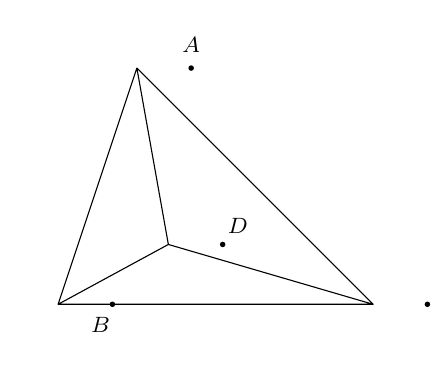
\begin{tikzpicture}[scale=1, font=\footnotesize, line join=round, line cap=round,>=stealth]
			\path
			(2,4) coordinate (A)
			(1,1) coordinate (B)
			(5,1) coordinate (C)
			(2.4,1.76) coordinate (D)
			;
			\draw (A)--(B)--(C)--(A)--(D)  (B)--(D)--(C);
			
			\tkzMarkAngle[arc=l, size=0.7cm,mark=0](B,A,D)
			\tkzLabelAngle[pos=1.1](B,A,D) {$\varphi$}
			\tkzMarkAngle[arc=l, size=0.7cm,mark=0](C,B,D)
			\tkzLabelAngle[pos=1.1](C,B,D) {$\varphi$}
			\tkzMarkAngle[arc=l, size=0.7cm,mark=0](A,C,D)
			\tkzLabelAngle[pos=1.1](A,C,D) {$\varphi$}
			\foreach \x/\g in {A/90,B/-120,C/-60,D/50} 
			\fill[black] (\x) circle (1pt)+(\g:3mm) node {$\x$};
		\end{tikzpicture}
	}
	\loigiai{
		Áp dụng định lí sin cho các tam giác $ABD$, $BCD$ và $ACD$ ta nhận được
		\[
		\heva{&\dfrac{BD}{\sin \varphi} = \dfrac{AD}{\sin (B- \varphi)}\\&  \dfrac{CD}{\sin \varphi} = \dfrac{BD}{\sin (C- \varphi)}\\&\dfrac{AD}{\sin \varphi} = \dfrac{CD}{\sin (A- \varphi)}} \Rightarrow \dfrac{BD}{\sin \varphi} \cdot \dfrac{CD}{\sin \varphi}  \cdot \dfrac{AD}{\sin \varphi} = \dfrac{AD}{\sin (B- \varphi)} \cdot \dfrac{BD}{\sin (C- \varphi)} \cdot \dfrac{CD}{\sin (A- \varphi)}.
		\]
		Rút gọn,  ta suy ra $\sin^3 \varphi = \sin (A- \varphi)  \sin (B- \varphi)   \sin (C- \varphi)$. 
	}
\end{bt}
\begin{dang}{Giải tam giác và ứng dụng}
	Giải tam giác là bài toán tìm độ dài tất cả các cạnh và độ lớn tất cả các góc của tam giác.
\end{dang}
\viduminhhoa
\begin{vd}%[Phạm Tuấn]%[0H2B3-1] 
	\immini{
		Cho tam giác $A B C$ có $BC=40\mathrm{~cm}$, $\widehat{B}=30^{\circ}, \widehat{C}=45^{\circ}$. Tính góc $\widehat{A}$ và độ dài các cạnh $A B$, $A C$  của tam giác đó (làm tròn kết quả đến hàng phần mười).
	}
	{
		\begin{tikzpicture}[scale=1, font=\footnotesize, line join=round, line cap=round,>=stealth]
			\path
			(0,0) coordinate (B)
			(4,0) coordinate (C)
			;
			\coordinate (B') at ($(B)+(30:3)$) ; 
			\coordinate (C') at ($(C)+(-45:3)$) ; 
			\coordinate (A) at (intersection of B--B' and C--C');
			\draw (A)--(B)--(C)--(A) ;
			
			\tkzMarkAngle[arc=ll,size=0.6,mark=0](C,B,A)
			\tkzLabelAngle[pos=.9](C,B,A) {$30^\circ$}
			\tkzMarkAngle[arc=l, size=0.6,mark=0](A,C,B)
			\tkzLabelAngle[pos=0.9](A,C,B) {$45^\circ$}
			\foreach \x/\g in {A/90,B/-120,C/-60} 
			\fill[black] (\x) circle (1pt)+(\g:3mm) node {$\x$};
		\end{tikzpicture}
	}
	\loigiai{
		Ta  có $\widehat{A} = 180^\circ - (\widehat{B}+\widehat{C}) = 180^\circ - (30^{\circ}+45^{\circ}) = 105^{\circ}$. \\
		Áp dụng định lí sin ta có 
		\begin{align*}
			&\dfrac{AB}{\sin C} = \dfrac{BC}{\sin A} \Rightarrow AB = \dfrac{BC\sin C}{\sin A}  = \dfrac{40\sin 45^{\circ}}{105^{\circ}} \approx 29{,}3 \mathrm{~(cm)}; \\
			&\dfrac{AC}{\sin B} = \dfrac{BC}{\sin A} \Rightarrow AC = \dfrac{BC\sin B}{\sin A}  = \dfrac{40\sin 30^{\circ}}{105^{\circ}} \approx 20{,}7 \mathrm{~(cm)}. 
		\end{align*}
	}
\end{vd}

\begin{vd}%[Phạm Tuấn]%[0H2B3-1] 
	Cho tam giác $ABC$ có $AB=25$, $AC=20$, $\widehat{A}=120^{\circ}$. Tính cạnh $BC$ và các góc $B$, $C$  của tam giác đó.  
	\loigiai{
		Áp dụng định lí côsin ta có 
		\[ BC^2=AB^2+AC^2-2AB \cdot AC \cos A =25^2+20^2-2 \cdot 25 \cdot 20 \cos 120^\circ  =  1525 \Rightarrow BC=5\sqrt{61} \approx 39.\]
		Áp dụng định lí sin ta có 
		\begin{align*}
			\dfrac{AC}{\sin B} = \dfrac{BC}{\sin A} \Rightarrow \sin B = \dfrac{AC\sin A}{BC}  = \dfrac{20 \sin 120^{\circ}}{5\sqrt{61}} \Rightarrow B \approx 26{,}3^\circ.  
		\end{align*}
		Khi đó $\widehat{C}= 180^\circ - \widehat{A} - \widehat{B} =  180^\circ  -120^\circ - 26{,}3^\circ= 33{,}7^\circ$.
	}
\end{vd}

\begin{vd}%[Phạm Tuấn]%[0H2B3-4]
	\immini{
		Để đo chiều rộng $AB$ của một khúc sông, người ta chọn điểm $C$.  Sau đó,  đo khoảng cách $BC$, các góc $B$ và $C$. Biết rằng $BC = 200$ m, $\widehat{B} = 107^\circ$,  $\widehat{C} = 28^\circ$. Tìm chiều rộng $AB$ của khúc sông đó (làm tròn đến chữ số thập phân thứ nhất).
	}
	{
		\begin{tikzpicture}[scale=1]
			\coordinate (X) at (1,1);
			\foreach \i in {0,...,6}
			\foreach \j  in {0,...,2}  
			\draw[blue] ($(X)+({\i+0.5},{0.6*(\j)+0.4})$)--($(X)+({\i+0.7},{0.6*(\j)+0.4})$);
			\coordinate [label=above left:$A$](A) at (3,3);
			\coordinate [label=below left:$B$](B) at (3,1);
			\coordinate [label=right:$C$](C) at (5,0.5);
			\draw (X)--(8,1) (8,3)--(1,3) (A)--(B)--(C)--(A);
			\foreach \i in {A,B,C} \draw[fill=black] (\i) circle(1.2pt);
		\end{tikzpicture}
	}
	\loigiai{
		Ta có $\widehat{A}= 180^\circ -  \widehat{B} -\widehat{C} =180^\circ- 107^\circ - 28^\circ=55^\circ$. \\
		Áp dụng định lí sin ta có 
		\[
		\dfrac{AB}{\sin C} = \dfrac{BC}{\sin A} \Rightarrow AB = \dfrac{BC\sin C}{\sin A}  = \dfrac{200\sin 28^{\circ}}{\sin 55^{\circ}} \approx 113{,}6\mathrm{~m}. 
		\]
	}
\end{vd}

\begin{vd}%[Phạm Tuấn]%[0H2B3-4]
	\immini{
		Để đo chiều cao $CH$ của một  tháp truyền hình, người ta chọn hai điểm quan sát $A$, $B$ trên mặt đất (hình vẽ).  Biết $\widehat{CAH} =51^\circ$, $\widehat{CBH} =66^\circ$ và $AB=75 \mathrm{~m}$, tính chiều cao của tháp.
	}
	{
		\begin{tikzpicture}[scale=1, font=\footnotesize, line join=round, line cap=round,>=stealth]
			\path
			(1,0) coordinate (A)
			(2,0) coordinate (B)
			(4,3.5) coordinate (C)
			(4,0) coordinate (H)
			(3.75,0) coordinate (U)
			(4.25,0) coordinate (V)
			;
			\draw[thick] (U)--(C)--(V); 
			\draw (B)--(C)--(A)--(V) ;
			\draw[dashed] (C)--(H) ;  
			\draw  
			($(C)!{1}!(U)$)--($(C)!{0.9}!(V)$)
			--($(C)!{0.8}!(U)$)--($(C)!{0.7}!(V)$)
			--($(C)!{0.6}!(U)$)--($(C)!{0.5}!(V)$)
			--($(C)!{0.4}!(U)$)--($(C)!{0.3}!(V)$)
			--($(C)!{0.2}!(U)$)--($(C)!{0.1}!(V)$)
			;
			
			\tkzMarkAngle[arc=l, size=0.6,mark=0](H,A,C)
			\tkzLabelAngle[pos=1](H,A,C) {$51^{\circ}$}
			\tkzMarkAngle[arc=ll, size=0.6,mark=0](H,B,C)
			\tkzLabelAngle[pos=1](H,B,C) {$66^{\circ}$}
			\foreach \x/\g in {A/-90,B/-90,C/90,H/-90} 
			\fill[black] (\x) circle (1pt)+(\g:3mm) node {$\x$};
		\end{tikzpicture}
	}
	
	\loigiai{
		Ta có $\widehat{ACB}=\widehat{CBH} - \widehat{CAH}=  66^\circ -51^\circ= 15^\circ$. \\
		Áp dụng định lí sin ta có
		\[
		\dfrac{AB}{\sin \widehat{ACB}} = \dfrac{BC}{\sin \widehat{CAH} } \Rightarrow BC = \dfrac{AB\sin \widehat{CAH}}{\sin \widehat{ACB}}  = \dfrac{75\sin 51^\circ}{\sin 15^\circ}.
		\]
		Suy ra $CH =BC\sin \widehat{CBH} = \dfrac{75 \sin 51^\circ \sin 66^\circ}{\sin 15^\circ} \approx 205{,}7\mathrm{~m}.$
	}
\end{vd}

\begin{vd}%[Phạm Tuấn]%[0H2B3-4]
	\immini{
		Trên ngọn đồi có một cái tháp cao $120 \mathrm{~m}$. Đỉnh tháp $B$ và chân tháp $C$ nhìn điểm $A$ ở chân đồi dưới các góc tương ứng bằng $35^{\circ}$ và $60^{\circ}$ so với phương thẳng đứng. Xác định chiều cao $H A$ của ngọn đồi. (Làm tròn đến phần mười)
	}
	{
		\begin{tikzpicture}[scale=1, font=\footnotesize, line join=round, line cap=round, >=stealth]
			\path 
			(0,0) coordinate (X)
			(1.1,2) coordinate (Y)
			(2,2) coordinate (Z)
			(5,0) coordinate (A)
			(1.5,5) coordinate (B)
			(1.5,2) coordinate (C)
			(1.5,0) coordinate (K)
			(1.3,2) coordinate (U)
			(1.8,2) coordinate (V) 
			(5,2) coordinate (H);
			\draw  
			($(B)!{1}!(U)$)--($(B)!{0.9}!(V)$)
			--($(B)!{0.8}!(U)$)--($(B)!{0.7}!(V)$)
			--($(B)!{0.6}!(U)$)--($(B)!{0.5}!(V)$)
			--($(B)!{0.4}!(U)$)--($(B)!{0.3}!(V)$)
			--($(B)!{0.2}!(U)$)--($(B)!{0.1}!(V)$)
			;
			\draw[thick]  (X)--(A)--(Z)--(Y)--(X);
			\draw (A)--(B)  (U)--(B)--(V) (Y)--($(Y)!{1.2}!(H)$)  (X)--($(X)!{1.2}!(A)$);
			\draw[->] (A)--(H) ; 
			\draw ($(A)!0.5!(H)$) node[right]{$h$};
			\draw[dashed](B)--(K) (A)--(C);
			
			\tkzMarkAngle[arc=l, size=0.6,mark=0](K,C,A)
			\tkzLabelAngle[pos=0.9](K,C,A) {$60^{\circ}$}
			\tkzMarkAngle[arc=ll, size=0.7,mark=0](K,B,A)
			\tkzLabelAngle[pos=1.1](V,B,A) {$35^{\circ}$}
			\foreach \x/\g in{A/-90,B/90,C/-130,H/90}
			\fill[black](\x) ($(\x)+(\g:3mm)$)node{$\x$}; 
		\end{tikzpicture}
	}
	\loigiai{
		Ta có $\widehat{BAC} = 60^\circ - 35^\circ =25^\circ $;  $\widehat{ACH} = 90^\circ - 60^\circ =30^\circ $\\
		Áp dụng định lí sin ta có
		\[
		\dfrac{AC}{\sin \widehat{ABC}} = \dfrac{BC}{\sin \widehat{BAC}} \Rightarrow AC =  \dfrac{BC\sin \widehat{ABC}}{\sin \widehat{BAC}}
		= \dfrac{120\sin 35^\circ}{\sin 25^\circ}.
		\]
		Suy ra $AH =AC \sin \widehat{ACH} = \dfrac{120 \sin 35^\circ \sin 30^\circ }{\sin 25^\circ} \approx 81{,}4 \mathrm{~m}$.
	}
\end{vd}
\baitaptl

\begin{bt}%[Phạm Tuấn]%[0H2B3-1]
	Cho tam giác $ABC$ có $AB=8$, $BC=10$, $AC=15$.  Tính $\widehat{A} + 2\widehat{C}$ (làm tròn kết quả đến hàng phần mười).
	\loigiai{
		Áp dụng định lí côsin ta có
		\begin{align*}
			&\cos A = \dfrac{AB^2+AC^2-BC^2}{2 \cdot AB \cdot AC} = \dfrac{8^2+15^2-10^2}{2 \cdot 8 \cdot 15 } = \dfrac{63}{80} \Rightarrow \widehat{A} \approx  38{,}04^\circ. \\
			&\cos C = \dfrac{AC^2+BC^2-AB^2}{2 \cdot AC \cdot BC} = \dfrac{15^2+10^2-8^2}{2 \cdot 15 \cdot 10 } = \dfrac{87}{100} \Rightarrow \widehat{C} \approx  29{,}54^\circ.
		\end{align*}
		Suy ra $\widehat{A} + 2\widehat{C} \approx 97{,}1^\circ$. 
	}
\end{bt}

\begin{bt}%[Phạm Tuấn]%[0H2B3-1]
	Cho tam giác $A B C$ có $AB=15\mathrm{~cm}$, $AC=21\mathrm{~cm}$, $\widehat{A}=30^{\circ}$. Tính cạnh $BC$ và các góc $B$, $C$  của tam giác đó (làm tròn kết quả đến hàng phần mười).
	\loigiai{
		Áp dụng định lí côsin ta có 
		\[ BC^2=AB^2+AC^2-2AB \cdot AC \cos A =15^2+21^2-2 \cdot 15 \cdot 21 \cos 30^\circ   \Rightarrow BC \approx 11 \mathrm{~cm}.\]
		Áp dụng định lí sin ta có 
		\begin{align*}
			\dfrac{AC}{\sin B} = \dfrac{BC}{\sin A} \Rightarrow \sin B = \dfrac{AC\sin A}{BC}  = \dfrac{21 \sin 30^{\circ}}{11} \Rightarrow B \approx 72{,}7^\circ.
		\end{align*}
		Khi đó $\widehat{C}= 180^\circ - \widehat{A}- \widehat{B}= 180^\circ - 30^\circ -72{,}7^\circ =77{,}3^\circ $.
	}
\end{bt}

\begin{bt}%[Phạm Tuấn]%[0H2K3-1] 
	\immini{
		Cho tam giác $A B C$ có $AB=15$, $AC=12$, $\widehat{A}=60^{\circ}$. $M$ là điểm thuộc cạnh $AB$  sao cho $AM=2BM$. Tính cạnh $CM$,  góc $\widehat{BCM}$ và bán kính đường tròn ngoại tiếp tam giác  $BCM$ (làm tròn kết quả đến hàng phần mười).
	}
	{
		\begin{tikzpicture}[scale=1, font=\footnotesize, line join=round, line cap=round,>=stealth]
			\path
			(0,0) coordinate (A)
			(4,0) coordinate (B)
			;
			\coordinate (M) at ($(A)!{2/3}!(B)$) ;
			\coordinate (C) at ($(A)+(60:3)$) ; 
			\draw (A)--(B)--(C)--(A) (C)--(M) ;
			
			\tkzMarkAngle[arc=l, size=0.6,mark=0](B,A,C)
			\tkzLabelAngle[pos=1](B,A,C) {$60^{\circ}$}
			\foreach \x/\g in {A/-120,B/-60,C/90,M/-90} 
			\fill[black] (\x) circle (1pt)+(\g:3mm) node {$\x$};
		\end{tikzpicture}
	}
	\loigiai{
		Ta có $AM=2BM \Rightarrow BM = \dfrac{1}{3}AB=5$ và $AM=\dfrac{2}{3}AB=10$. \\
		Áp dụng định lí côsin ta có 
		\begin{align*}
			&CM^2=AM^2+AC^2-2AM \cdot AC \cos A =10^2+12^2-2 \cdot 10 \cdot 12 \cos 60^\circ  =  124 \Rightarrow CM=\sqrt{124} \approx 11{,}1; \\
			&BC^2=AB^2+AC^2-2AB \cdot AC \cos A =15^2+12^2-2 \cdot 15 \cdot 12 \cos 60^\circ  =  189\Rightarrow BC=\sqrt{189}.
		\end{align*}
		Áp dụng định lí côsin ta có 
		\begin{align*}
			&BM^2=CM^2+CB^2-2CM \cdot CB \cos \widehat{BCM}  \\
			\Leftrightarrow~ & \cos \widehat{BCM} = \dfrac{CM^2+CB^2- BM^2}{2CM \cdot CB}  \\
			\Leftrightarrow~ & \cos \widehat{BCM} = \dfrac{124+189- 5^2}{2\sqrt{124} \cdot \sqrt{189}}  \\
			\Rightarrow~& \widehat{BCM} \approx 19{,}8^\circ. 
		\end{align*}
		Áp đụng định lí sin,  ta nhận được bán kính đường tròn ngoại tiếp tam giác $BCM$ là
		\[
		R = \dfrac{BM}{2\sin \widehat{BCM}} \approx 7{,}4. 
		\]
	}
\end{bt}

\begin{bt}%[Phạm Tuấn]%[0H2B3-4]
	\immini{
		Để đo chiều rộng $AB$ của một khúc sông, người ta chọn điểm $C$,  đo khoảng cách $BC$, các góc $B$ và $C$. Biết rằng $BC = 250$ m, $\widehat{B} = 104^\circ$,  $\widehat{C} = 31^\circ$. Tìm chiều rộng $AB$ của khúc sông đó (làm tròn đến chữ số hàng đơn vị).
	}
	{
		\begin{tikzpicture}[scale=1, font=\footnotesize, line join=round, line cap=round,>=stealth]
			\coordinate (X) at (1,1);
			\foreach \i in {0,...,6}
			\foreach \j  in {0,...,2}  
			\draw[blue] ($(X)+({\i+0.5},{0.6*(\j)+0.4})$)--($(X)+({\i+0.7},{0.6*(\j)+0.4})$);
			\coordinate [label=above:$A$](A) at (3,3);
			\coordinate [label=below:$B$](B) at (3,1);
			\coordinate [label=right:$C$](C) at (5,0.5);
			\draw (X)--(8,1) (8,3)--(1,3) (A)--(B)--(C)--(A);
			\foreach \i in {A,B,C} \draw[fill=black] (\i) circle(1.2pt);
		\end{tikzpicture}
	}
	\loigiai{
		Ta có $\widehat{A}= 180^\circ -  \widehat{B} -\widehat{C} =180^\circ- 104^\circ - 31^\circ=45^\circ$. \\
		Áp dụng định lí sin ta có 
		\[
		\dfrac{AB}{\sin C} = \dfrac{BC}{\sin A} \Rightarrow AB = \dfrac{BC\sin C}{\sin A}  = \dfrac{250\sin 31^{\circ}}{\sin 45^{\circ}} \approx 182 \mathrm{~m}. 
		\]
	}
\end{bt}

\begin{bt}%[Phạm Tuấn]%[0H2B3-4]
	\immini{
		Để đo chiều cao $CH$ của một  tháp truyền hình, người ta chọn hai điểm quan sát $A$, $B$ trên mặt đất (hình vẽ).  Biết $\widehat{CAH} =54^\circ$, $\widehat{CBH} =68^\circ$ và $AB=80 \mathrm{~m}$, tính chiều cao của tháp (Làm tròn đến hàng đơn vị).
	}
	{
		\begin{tikzpicture}[scale=1, font=\footnotesize, line join=round, line cap=round,>=stealth]
			\path
			(1,0) coordinate (A)
			(2,0) coordinate (B)
			(4,3.5) coordinate (C)
			(4,0) coordinate (H)
			(3.75,0) coordinate (U)
			(4.25,0) coordinate (V)
			;
			\draw[thick] (U)--(C)--(V); 
			\draw (B)--(C)--(A)--(V) ;
			\draw[dashed] (C)--(H) ;  
			\draw  
			($(C)!{1}!(U)$)--($(C)!{0.9}!(V)$)
			--($(C)!{0.8}!(U)$)--($(C)!{0.7}!(V)$)
			--($(C)!{0.6}!(U)$)--($(C)!{0.5}!(V)$)
			--($(C)!{0.4}!(U)$)--($(C)!{0.3}!(V)$)
			--($(C)!{0.2}!(U)$)--($(C)!{0.1}!(V)$)
			;
			
			\tkzMarkAngle[arc=l, size=0.6,mark=0](H,A,C)
			\tkzLabelAngle[pos=1](H,A,C) {$54^{\circ}$}
			\tkzMarkAngle[arc=ll, size=0.6,mark=0](H,B,C)
			\tkzLabelAngle[pos=1](H,B,C) {$68^{\circ}$}
			\foreach \x/\g in {A/-90,B/-90,C/90,H/-90} 
			\fill[black] (\x) circle (1pt)+(\g:3mm) node {$\x$};
		\end{tikzpicture}
	}
	
	\loigiai{
		Ta có $\widehat{ACB}=\widehat{CBH} - \widehat{CAH}=  68^\circ -54^\circ= 14^\circ$. \\
		Áp dụng định lí sin ta có
		\[
		\dfrac{AB}{\sin \widehat{ACB}} = \dfrac{BC}{\sin \widehat{CAH} } \Rightarrow BC = \dfrac{AB\sin \widehat{CAH}}{\sin \widehat{ACB}}  = \dfrac{80\sin 54^\circ}{\sin 14^\circ}.
		\]
		Suy ra $CH =BC\sin \widehat{CBH} = \dfrac{80 \sin 54^\circ \sin 68^\circ}{\sin 14^\circ} \approx 248 \mathrm{~m}.$
	}
\end{bt}
\begin{dang}{Bài tập tổng hợp}
	
\end{dang}
\viduminhhoa
\begin{vd}%[Chim Khuyên]%[0H2B3-1] 
	Cho tam giác $ABC$ có $\widehat{A}= 60^\circ$ và $AB= 8 \mathrm{~cm}$, $AC= 5 \mathrm{~cm}$. 
	\begin{enumerate}
		\item Tính diện tích của tam giác $ABC$.
		\item Tính độ dài đường cao hạ từ đỉnh $A$ của tam giác $ABC$.
		\item Tính bán kính đường tròn nội tiếp tam giác $ABC$.
	\end{enumerate}
	\loigiai{
		\begin{center}
			\begin{tikzpicture}[scale=1, font=\footnotesize, line join=round, line cap=round,>=stealth]
				\path
				(0,0) coordinate (B)
				(5,0) coordinate (C)
				(3,2) coordinate (A)
				($(B)!(A)!(C)$) coordinate (H)
				;
				\draw (A)--(B)--(C)--(A)--(H);
				\draw pic["$60^{\circ}$", draw=black, angle eccentricity=1.5, angle radius=0.5cm]{angle=B--A--C} ;
				\foreach \x/\g in {A/90,B/-120,C/-60,H/-60} 
				\fill[black] (\x) circle (1pt)+(\g:3mm) node {$\x$};
			\end{tikzpicture}
		\end{center}
		\begin{enumerate}
			\item Áp dụng công thức tính diện tích tam giác ta có\\
			$S_{\triangle ABC}=\dfrac{1}{2}AB\cdot AC \cdot \sin 60^{\circ} = \dfrac{1}{2} \cdot 8 \cdot 5 \cdot \dfrac{\sqrt{3}}{2} = 10\sqrt{3} \mathrm{~cm}^2$. 
			\item Áp dụng định lí cosin trong tam giác $ABC$ ta có \\
			$BC^2= AB^2+AC^2-2 AB\cdot AC \cdot \cos 60^{\circ}= 8^2+5^2-2 \cdot 8\cdot 5 \cdot \dfrac{1}{2} =49 \Rightarrow BC=7$.\\
			$S_{\triangle ABC}=\dfrac{1}{2} AH \cdot BC \Rightarrow AH=\dfrac{2S_{\triangle ABC}}{BC}=\dfrac{2\cdot 10 \sqrt{3}}{7}=\dfrac{20\sqrt{3}}{7} $.
			\item $S_{\triangle  ABC}=pr \Rightarrow r=\dfrac{S_{\triangle  ABC}}{p}=\dfrac{2S_{\triangle  ABC}}{AB+BC+AC}=\dfrac{2 \cdot 10\sqrt{3}}{5+8+7}=\sqrt{3}$.
		\end{enumerate}
	}
\end{vd}
\begin{vd}%[Chim Khuyên]%[0H2B3-1] 
	Cho hình bình hành $ABCD$ có $AB=6, BC=8$ và $\widehat{ABC}=60^{\circ}$. Tính diện tích hình bình hành $ABCD$.
	\loigiai{
		\immini{Ta có \\
			$S_{ABCD}=2S_{\triangle ABC}=2\cdot \dfrac{1}{2} BA \cdot BC \cdot \cos \widehat{ABC} $\\
			$= 6\cdot 8 \cdot \cos 60^{\circ} =24$}{	\begin{tikzpicture}[line cap=round,line join=round, >=stealth,scale=.7]
				\tkzDefPoints{0/0/O,-2/1/A} 
				\coordinate (D) at ($(A)+(6,0)$);
				\tkzDefPointBy[homothety = center O ratio -1](A) \tkzGetPoint{C}   
				\tkzDefPointBy[homothety = center O ratio -1](D) \tkzGetPoint{B}  
				\tkzDrawSegments(A,B B,C C,D D,A) 
				\tkzLabelPoints[left](A,B) 
				\tkzLabelPoints[right](C,D)  
		\end{tikzpicture}}
	}
\end{vd}

\begin{vd}%[Chim Khuyên]%[0H2K3-1] 
	Cho tam giác $ABC$ có $\widehat{A}=120^\circ$, $\widehat{B}=30^\circ$, diện tích tam giác $ABC$ bằng $9\sqrt{3}$. Tính các cạnh của tam giác $ABC$.
	\loigiai
	{
		\immini
		{
			Ta có $\widehat{C}=180^\circ-(\widehat{A}+\widehat{B})=30^\circ$.\\
			Khi đó
			\allowdisplaybreaks
			\begin{eqnarray*}
				&&\heva{& \dfrac{BC}{\sin 120^\circ}=\dfrac{AC}{\sin 30^\circ}=\dfrac{AB}{\sin 30^\circ}\\ & S_{\triangle ABC}=\dfrac{1}{2}\cdot BC\cdot AC\cdot \sin 30^\circ=9\sqrt{3}}\\ &\Leftrightarrow&\heva{& BC=\sqrt{3}AC \\ &BC\cdot AC=36\sqrt{3}\\ &AC=AB} \Leftrightarrow \heva{& BC=6\sqrt{3}  \\ & AC=6\\ &AB=6.}
			\end{eqnarray*}
			Vậy $BC=6\sqrt{3}$, $AC=6$, $AB=6$.
		}
		{
			\begin{tikzpicture}[>=stealth,line join=round,line cap=round,line width=0.6pt,font=\footnotesize,scale=1]
				\coordinate[label=below left:$A$](A) at (0,0);
				\coordinate[label=below right:$B$](B) at (3,0);
				\coordinate [label=above right:$C$](C) at ($(A)!1!120:(B)$); % Quay hướng 60 độ và vị tự tỉ số 1 điểm B tâm A thành điểm B1
				\draw (A)--(B)--(C)--cycle;
				\foreach \x in {C,A,B}\draw[->] pic[draw,blue,angle radius=3mm] {angle = B--A--C};
				\foreach \x in {A,B,C} \fill (\x) circle (1.5pt) ;
				\draw (100:0.7)node[below right]{$120^\circ$};
			\end{tikzpicture}
		}
	}
\end{vd}
\begin{vd}%[Chim Khuyên]%[0H2K3-1]
	Cho tam giác $ABC$ có $AB=2$, $AC=2\sqrt{7}$ và $BC=4$.
	\begin{enumerate}
		\item Tính góc $B$ và diện tích tam giác $ABC$.
		\item Tính độ dài đường phân giác trong của góc $B$ của tam giác $ABC$.
	\end{enumerate}
	\loigiai
	{
		\immini
		{
			\begin{enumerate}
				\item Ta có $\cos B=\dfrac{AB^2+BC^2-AC^2}{2\cdot AB \cdot BC}= \dfrac{4+16-28}{2\cdot 2 \cdot 4}=\dfrac{-1}{2} \Rightarrow \widehat{B}= 120^\circ$.\\
				Và $S_{\triangle ABC}=\dfrac{1}{2}AB\cdot BC\cdot \sin 120^\circ=2\sqrt{3}$.
				\item Gọi $D$ là chân đường phân giác trong của góc $B$.\\
				Ta có
				\allowdisplaybreaks
				\begin{eqnarray*}
					&&S_{\triangle ABC} = S_{\triangle ABD} + S_{\triangle BCD}\\ &\Leftrightarrow& 2\sqrt{3}=\dfrac{1}{2} AB \cdot BD \cdot \sin \widehat{ABD} +\dfrac{1}{2} CB \cdot BD \cdot \sin \widehat{CBD}\\
					&\Leftrightarrow& 2\sqrt{3}=\dfrac{1}{2} \cdot 2 \cdot BD \cdot \sin 60^\circ +\dfrac{1}{2}\cdot 4 \cdot BD \cdot \sin 60^\circ\\
					&\Leftrightarrow & 2\sqrt{3} = \dfrac{3\sqrt{3}}{2}BD\Leftrightarrow BD= \dfrac{4}{3}.
				\end{eqnarray*}
			\end{enumerate}
		}
		{
			\begin{tikzpicture}[>=stealth,line join=round,line cap=round,line width=0.6pt,font=\footnotesize]
				\coordinate[label=below left:$B$](B) at (0,0);
				\coordinate[label=below right:$C$](C) at (4,0);
				\coordinate [label=above right:$A$](A) at ($(B)!0.5!120:(C)$); 
				\coordinate [label=above  right:$D$](D) at ($(B)!0.333!60:(C)$);
				\draw (A)--(B)--(C)--cycle (B)--(D);
				\foreach \x in {A,B,C,D} \fill (\x) circle (1.5pt) ;
				\draw pic[draw,blue,angle radius=4mm] {angle = D--B--A} ($($(B)!4mm!(A)$)!.5!($(B)!4mm!(D)$)$)node[rotate=180]{\scriptsize $|$}; 
				\draw pic[draw,blue,angle radius=4mm] {angle = C--B--D} ($($(B)!4mm!(C)$)!.5!($(B)!4mm!(D)$)$)node[rotate=120]{\scriptsize $|$}; 
				
			\end{tikzpicture}
		}
	}
\end{vd}

\baitaptl

\begin{bt}%[Chim Khuyên]%[0H2B2-8]
	Cho tam giác với ba cạnh $ a=13,b=14,c=15$. Tính diện tích của tam giác và độ dài đường cao $ h_c$.
	\loigiai{
		Ta có $ S=\sqrt{p(p-a)(p-b)(p-c)}=84$
		Lại có 
		$ S=\dfrac{1}{2}h_c \cdot 15 \Rightarrow h_c=11\dfrac{1}{5}. $	
	}
	
\end{bt}

\begin{bt}%[Chim Khuyên]%[0H2K3-1]
	Cho tam giác $ABC$ có $AB=10$, $BC=6$ và góc $\widehat{B}=120^\circ$.
	\begin{enumerate}
		\item Tính $AC$ và diện tích tam giác $ABC$.
		\item Tính đường cao $AH$ và bán kính đường tròn nội tiếp tam giác $ABC$.
		\item Tính độ dài đường phân giác trong $BD$ của tam giác $ABC$.
	\end{enumerate}
	
	\loigiai{
		\begin{enumerate}
			\item Ta có $AC= \sqrt{AB^2+BC^2-2AB\cdot BC \cdot \cos B}=14$
			và $S_{\triangle ABC}=\dfrac{1}{2}\cdot AB \cdot BC \cdot \sin B=15\sqrt{3}$.
			\item Ta có 
			\immini
			{
				$AH=\dfrac{2S_{\triangle ABC}}{BC}=\dfrac{2\cdot 15\sqrt{3}}{14}$\\ và $r=\dfrac{S_{\triangle ABC}}{p}=\dfrac{15\sqrt{3}}{15}=\sqrt{3}$ với $p=\dfrac{6+10+14}{2}=15$.
			}
			{
				\begin{tikzpicture}[>=stealth,line join=round,line cap=round,line width=0.6pt,font=\footnotesize]
					\coordinate[label=below left:$B$](B) at (0,0);
					\coordinate[label=below right:$C$](C) at (3,0);
					\coordinate [label=above right:$A$](A) at ($(B)!1.2!120:(C)$); 
					\coordinate [label=above  right:$D$](D) at ($(B)!0.545!60:(C)$);
					\draw (A)--(B)--(C)--cycle (B)--(D);
					\foreach \x in {A,B,C,D} \fill (\x) circle (1.5pt) ;
					\draw pic[draw,blue,angle radius=4mm] {angle = D--B--A} ($($(B)!4mm!(A)$)!.5!($(B)!4mm!(D)$)$)node[rotate=180]{\scriptsize $|$}; 
					\draw pic[draw,blue,angle radius=4mm] {angle = C--B--D} ($($(B)!4mm!(C)$)!.5!($(B)!4mm!(D)$)$)node[rotate=120]{\scriptsize $|$}; 
					
				\end{tikzpicture}
			}
			\item  Ta có
			\allowdisplaybreaks
			\begin{eqnarray*}
				&&S_{\triangle ABC} = S_{\triangle ABD} + S_{\triangle BCD}\\ &\Leftrightarrow& 15\sqrt{3}=\dfrac{1}{2} AB \cdot BD \cdot \sin \widehat{ABD} +\dfrac{1}{2} CB \cdot BD \cdot \sin \widehat{CBD}\\
				&\Leftrightarrow& 15\sqrt{3}=\dfrac{1}{2}\cdot 10 \cdot BD \cdot \sin 60^\circ +\dfrac{1}{2} \cdot 6 \cdot BD \cdot \sin 60^\circ\\
				&\Leftrightarrow&15\sqrt{3}=4\sqrt{3}\cdot BD\Leftrightarrow BD= \dfrac{15}{4}.
			\end{eqnarray*}
	\end{enumerate}	}
\end{bt}

\begin{bt}%[ Chim Khuyên]%[0H2K3-1]
	Cho tam giác $ABC$ có $AB=2$, $AC=3$ và $\widehat{BAC}=120^\circ$. Tính độ dài $BC$, diện tích tam giác $ABC$, độ dài đường phân giác trong $AD$ của tam giác $ABC$.
	\loigiai
	{
		\immini
		{
			Ta có 
			\begin{itemize}
				\item[$\bullet$] $BC= \sqrt{AB^2+AC^2-2AB\cdot AC \cdot \cos A}=\sqrt{19}$\\ và $S_{\triangle ABC}=\dfrac{1}{2}AB\cdot AC \sin A=\dfrac{3\sqrt{3}}{2}$.
				\item  [$\bullet$] Và 
				\allowdisplaybreaks
				\begin{eqnarray*}
					&&S_{\triangle ABC} = S_{\triangle BAD} + S_{\triangle DAC}\\ &\Leftrightarrow& \dfrac{ 3\sqrt{3}}{2}=\dfrac{1}{2} AB \cdot AD \cdot \sin \widehat{BAD} +\dfrac{1}{2} AC \cdot AD \cdot \sin \widehat{DAC}\\
					&\Leftrightarrow& \dfrac{ 3\sqrt{3}}{2}=\dfrac{1}{2} \cdot 2 \cdot AD \cdot \sin 60^\circ +\dfrac{1}{2}\cdot 3 \cdot AD \cdot \sin 60^\circ\\
					&\Leftrightarrow & \dfrac{ 3\sqrt{3}}{2} = \dfrac{5\sqrt{3}}{4}AD\Leftrightarrow AD= \dfrac{6}{5}.
				\end{eqnarray*}
			\end{itemize}
			
		}
		{
			\begin{tikzpicture}[>=stealth,line join=round,line cap=round,line width=0.6pt,font=\footnotesize,scale=1.3]
				\coordinate[label=below left:$A$](A) at (0,0);
				\coordinate[label=below right:$C$](C) at (3,0);
				\coordinate [label=above right:$B$](B) at ($(A)!0.5!120:(C)$); 
				\coordinate [label=above  right:$D$](D) at ($(A)!0.333!60:(C)$);
				\draw (A)--(B)--(C)--cycle (A)--(D);
				\foreach \x in {A,B,C,D} \fill (\x) circle (1.5pt) ;
				\draw pic[draw,blue,angle radius=4mm] {angle = D--A--B} ($($(A)!3mm!(B)$)!.5!($(A)!3mm!(D)$)$)node[rotate=180]{\scriptsize $|$}; 
				\draw pic[draw,blue,angle radius=4mm] {angle = C--A--D} ($($(A)!3mm!(C)$)!.5!($(A)!3mm!(D)$)$)node[rotate=120]{\scriptsize $|$}; 
				
			\end{tikzpicture}
		}
	}
\end{bt}

\begin{bt}%[Chim Khuyên]%[0H2K3-2]
	Cho tam giác $ABC$ có $AB=c$, $BC=a$, $AC=b$. Gọi $h_a$, $h_b$, $h_c$ lần lượt là các đường cao tương ứng xuất phát từ các đỉnh $A$, $B$, $C$ và $r$ là bán kính đường tròn nội tiếp tam giác $ABC$. Chứng minh $\dfrac{1}{h_a}+\dfrac{1}{h_b}+\dfrac{1}{h_c}=\dfrac{1}{r}$.
	\loigiai{
		Ta có $S=\dfrac{1}{2}ah_a=\dfrac{1}{2}bh_b=\dfrac{1}{2}ch_c \Rightarrow \dfrac{1}{h_a}=\dfrac{a}{2S},\dfrac{1}{h_b}=\dfrac{b}{2S}, \dfrac{1}{h_c}=\dfrac{c}{2S}$ và $S=pr \Rightarrow \dfrac{1}{r}=\dfrac{p}{S}$.
		{\allowdisplaybreaks
			\begin{eqnarray*}
				VT=\dfrac{1}{h_a}+\dfrac{1}{h_b}+\dfrac{1}{h_c}&=&\dfrac{a}{2S}+\dfrac{b}{2S}+\dfrac{c}{2S}\\
				&=&\dfrac{a+b+c}{2S}=\dfrac{2p}{2S}\\
				&=&\dfrac{p}{S}=\dfrac{1}{r}.
		\end{eqnarray*}}
	}
\end{bt}

\begin{bt}%[Chim Khuyên]%[0H2K2-2]
	Cho tam giác $ABC$ không vuông ở $A$, chứng minh $S=\dfrac{1}{4}\left(b^2+c^2-a^2\right)\tan A$.
	\loigiai{
		Ta có 
		{\allowdisplaybreaks
			\begin{eqnarray*}
				S&=&\dfrac{1}{2}bc\sin A\\
				&=&\dfrac{1}{2}bc\cos A \cdot \dfrac{\sin A}{\cos A}\\
				&=&\dfrac{1}{2}bc\cdot \dfrac{b^2+c^2-a^2}{2bc} \cdot \tan A\\
				&=&\dfrac{1}{4}\left(b^2+c^2-a^2\right) \cdot \tan A.	
		\end{eqnarray*}}	
	}
\end{bt}
\subsection{Câu hỏi trắc nghiệm}
	\Opensolutionfile{ansbook}[ans/ansbook-0D3-6-TN]
	\Opensolutionfile{ans}[ans/ans-0D3-6-TN]
	\begin{ex}%[0H2Y3-1]
		Tam giác $ ABC$ có $ AB=5$, $BC=7$, $CA=8$. Số đo góc $ \widehat{A}$ bằng
		\choice
		{$ 90^\circ $}
		{$ 45^\circ $}
		{\True $ 60^\circ $}
		{$ 30^\circ $}
		\loigiai
		{Theo định lí hàm cosine, ta có $ \cos{A}=\dfrac{AB^2+AC^2-BC^2}{2AB\cdot AC}=\dfrac{5^2+8^2-7^2}{2\cdot 5\cdot 8}=\dfrac{1}{2}$.\\
			Do đó, $ \widehat{A}=60^\circ $.}
	\end{ex}
	\begin{ex}%[0H2Y3-1]
		Tam giác $ ABC$ có $ AB=\sqrt{2}$, $AC=\sqrt{3}$ và $ \widehat{C}=45^\circ $. Tính độ dài cạnh $ BC$.
		\choice
		{$ BC=\sqrt{5}$}
		{\True $ BC=\dfrac{\sqrt{6}+\sqrt{2}}{2}$}
		{$ BC=\sqrt{6}$}
		{$ BC=\dfrac{\sqrt{6}-\sqrt{2}}{2}$}
		\loigiai
		{Theo định lí hàm cosine, ta có\\
			$ AB^2=AC^2+BC^2-2\cdot AC\cdot BC\cdot \cos \widehat{C}\Rightarrow {(\sqrt{2} )}^2={(\sqrt{3} )}^2+BC^2-2\cdot \sqrt{3}\cdot BC\cdot \cos 45^\circ $ \\
			$ \Rightarrow BC=\dfrac{\sqrt{6}+\sqrt{2}}{2}$.}
	\end{ex}
	\begin{ex}%[0H2Y3-1]
		Tam giác $ ABC$ có $ AB=2$, $AC=1$ và $ \widehat{A}=60^\circ $. Tính độ dài cạnh $ BC$.
		\choice
		{$ BC=\sqrt{2}$}
		{\True $ BC=\sqrt{3}$}
		{$ BC=1$}
		{$ BC=2$}
		\loigiai
		{Theo định lí hàm cosine, ta có\\
			$ BC^2=AB^2+AC^2-2AB\cdot AC\cdot \cos{A}=2^2+1^2-2\cdot 2\cdot 1\cdot \cos 60^\circ =3$\\
			$\Rightarrow BC=\sqrt{3}$.}
	\end{ex}
	\begin{ex}%[0H2B3-1]
		Tam giác $ ABC$ có $ AB=3$, $AC=6$, $\widehat{BAC}=60^\circ $. Tính độ dài đường cao $ h_a$ của tam giác.
		\choice
		{$ h_a=3\sqrt{3}$}
		{$ h_a=\sqrt{3}$}
		{$ h_a=\dfrac{3}{2}$}
		{\True $ h_a=3$}
		\loigiai
		{Áp dụng định lý hàm số cosine, ta có
			$ BC^2=AB^2+AC^2-2AB\cdot AC\cos A=27\Rightarrow BC=3\sqrt{3}$.\\
			Ta có $ S_{\Delta ABC}=\dfrac{1}{2}\cdot AB\cdot AC\cdot \sin{A}=\dfrac{1}{2}\cdot 3\cdot 6\cdot \sin 60^\circ=\dfrac{9\sqrt{3}}{2}$.\\
			Lại có $ S_{\Delta ABC}=\dfrac{1}{2}\cdot BC\cdot h_a\Rightarrow h_a=\dfrac{2S}{BC}=3$.}
	\end{ex}
	\begin{ex}%[0H2B3-1]
		Tam giác $ ABC$ có $ AB=\dfrac{\sqrt{6}-\sqrt{2}}{2}$, $BC=\sqrt{3}$, $CA=\sqrt{2}$. Gọi $ D$ là chân đường phân giác trong góc $ \widehat{A}$. Khi đó góc $ \widehat{ADB}$ bằng
		\choice
		{$ 90^\circ $}
		{$ 45^\circ $}
		{$ 60^\circ $}
		{\True $ 75^\circ $}
		\loigiai{
			\immini
			{
				Theo định lí hàm cosine, ta có\\
				$ \begin{aligned}
					& \cos \widehat{BAC}=\dfrac{AB^2+AC^2-BC^2}{2\cdot AB\cdot AC}=-\dfrac{1}{2}. \\
					\Rightarrow& \widehat{BAC}=120^\circ \Rightarrow \widehat{BAD}=60^\circ. \\
				\end{aligned}$ \\
				$ \begin{aligned}
					& \cos \widehat{ABC}=\dfrac{AB^2+BC^2-AC^2}{2\cdot AB\cdot BC}=\dfrac{\sqrt{2}}{2}.\\
					\Rightarrow &\widehat{ABC}=45^\circ.
				\end{aligned}$ \\
				Trong $ \Delta ABD$ có $ \widehat{BAD}=60^\circ$, $\widehat{ABD}=45^\circ. \\
				\Rightarrow \widehat{ADB}=75^\circ $.
			}
			{
				\begin{tikzpicture}[scale=1, font=\footnotesize, line join = round, line cap = round,>=stealth]
					\tkzDefPoints{-2/0/B,0/3/A,5/0/C}
					\clip (-2.2,-0.5) rectangle (5.2,3.5);
					\tkzInCenter(A,B,C) \tkzGetPoint{I}
					\tkzInterLL(A,I)(C,B) \tkzGetPoint{D}
					\tkzDrawPoints[fill=black](A,B,C,D)
					\tkzDrawPolygon(A,B,C)
					\tkzDrawSegments(D,A)
					\tkzLabelPoints[above](A)
					\tkzLabelPoints[below](D,B,C)
					\tkzMarkAngles[size=0.5cm,arc=l,mark=||](B,A,D D,A,C)
				\end{tikzpicture}
			}
		}
	\end{ex}
	\begin{ex}%[0H2B3-1]
		Tam giác $ ABC$ có $ AB=4$, $BC=6$, $AC=2\sqrt{7}$. Điểm $ M$ thuộc đoạn $ BC$ sao cho $ MC=2MB$. Tính độ dài cạnh $ AM$.
		\choice
		{$ AM=4\sqrt{2}$}
		{$ AM=3\sqrt{2}$}
		{\True $ AM=2\sqrt{3}$}
		{$ AM=3$}
		\loigiai{
			\immini
			{
				Theo định lí hàm cosine, ta có\\
				$ \cos B=\dfrac{AB^2+BC^2-AC^2}{2\cdot AB\cdot BC}=\dfrac{4^2+6^2-(2\sqrt{7} )^2}{2\cdot 4\cdot 6}=\dfrac{1}{2}$.\\
				Do $ MC=2MB\Rightarrow BM=\dfrac{1}{3}BC=2$.\\
				Theo định lí hàm cosine, ta có\\
				$ \begin{aligned}
					AM^2&=AB^2+BM^2-2\cdot AB\cdot BM\cdot \cos B \\
					& =4^2+2^2-2\cdot 4\cdot 2\cdot \dfrac{1}{2}=12.
				\end{aligned}\\
				\Rightarrow AM=2\sqrt{3}$.
			}
			{
				\begin{tikzpicture}[scale=0.9, font=\footnotesize, line join = round, line cap = round,>=stealth]
					\tkzDefPoints{-2/0/B,0/3/A,5/0/C}
					\coordinate (M) at ($(B)!0. 33!(C)$);
					\tkzDrawPoints[fill=black](A,B,C,M)
					\tkzDrawPolygon(A,B,C)
					\tkzDrawSegments(M,A)
					\tkzLabelPoints[above](A)
					\tkzLabelPoints[below](M,B,C)
				\end{tikzpicture}
		}}
	\end{ex}
	\begin{ex}%[0H2B3-1]
		Cho hình thoi $ ABCD$ cạnh bằng $ 1$ cm và có $ \widehat{BAD}=60^\circ $. Tính độ dài cạnh $ AC$.
		\choice
		{$ AC=2$}
		{\True $ AC=\sqrt{3}$}
		{$ AC=2\sqrt{3}$}
		{$ AC=\sqrt{2}$}
		\loigiai{
			\immini{
				Do $ ABCD$ là hình thoi, có $ \widehat{BAD}=60^\circ \Rightarrow \widehat{ABC}=120^\circ $.\\
				Theo định lí hàm cosine, ta có\\
				$ \begin{aligned}
					AC^2&=AB^2+BC^2-2\cdot AB\cdot BC\cdot \cos \widehat{ABC} \\
					& =1^2+1^2-2\cdot 1\cdot 1\cdot \cos 120^\circ\\
					& =3.\\
					\Rightarrow AC=\sqrt{3}\cdot \\
				\end{aligned}$}
			{
				\begin{tikzpicture}[scale=1, font=\footnotesize, line join = round, line cap = round,>=stealth]
					\tkzDefPoints{-2/0/A,0/3/B}
					\tkzDefPointBy[rotation = center A angle -60](B) \tkzGetPoint{D}
					\coordinate (C) at ($(B)+(D)-(A)$);
					\tkzDrawPoints[fill=black](A,B,C,D)
					\tkzDrawPolygon(A,B,C,D)
					\tkzDrawSegments(C,A D,B)
					\tkzLabelPoints[above](B,C)
					\tkzLabelPoints[below](A,D)
					\tkzMarkAngles[size=0.5cm,arc=l](D,A,B)
			\end{tikzpicture}}
		}
	\end{ex}
	\begin{ex}%[0H2B3-4]
		Khoảng cách từ $A$ đến $B$ không thể đo trực tiếp được vì phải qua một đầm lầy. Người ta xác định được một điểm $C$ mà từ đó có thể nhìn được $A$ và $B$ dưới một góc $78^\circ 24'$. Biết $CA=250$ m, $CB=120$ m. Khoảng cách $AB$ bằng bao nhiêu?
		\choice
		{$266$ m}
		{\True $255$ m}
		{$166$ m}
		{$298$ m}
		\loigiai{
			\immini
			{
				Áp dụng định lí cosine cho $\triangle ABC$, ta có
				$
				\begin{aligned}
					AB^2& =CA^2+CB^2-2CA\cdot CB\cdot \cos C\\
					& =250^2+120^2-2\cdot 250\cdot 120\cdot \cos 78^\circ 24'\\
					& \approx 64835
				\end{aligned}$.\\
				$\Rightarrow AB\approx 255$ (m).
			}
			{
				\begin{tikzpicture}[scale=1, font=\footnotesize, line join=round, line cap=round,>=stealth]
					\tkzInit[xmin=-1,xmax=7,ymin=-1,ymax=3.5]
					\tkzClip
					\tkzDefPoints{0/0/A,6/0/B}
					\tkzDefPointBy[rotation= center A angle 28](B) \tkzGetPoint{a}
					\tkzDefPointBy[rotation= center B angle -74](A) \tkzGetPoint{b}
					\tkzInterLL(A,a)(B,b) \tkzGetPoint{C}
					\tkzDrawPoints[fill=black](A,B,C)
					\tkzDrawSegments(A,B B,C C,A)
					\tkzLabelPoints[above](C) \tkzLabelPoints[above left](A)
					\tkzLabelPoints[above right](B)
					\draw[pattern = north west lines] (2,-0.0) parabola bend (3,-0.75) (4,-0.0)--cycle;
					\tkzLabelSegment[above left](A,C){$250$ m}
					\tkzLabelSegment[above right](C,B){$120$ m}
					\tkzLabelAngle[pos=.8](A,C,B){$78^{\circ}24'$}
					\tkzMarkAngle[size=.5](A,C,B)
				\end{tikzpicture}
			}	
		}
	\end{ex}
	\begin{ex} Cho tam giác $ABC$ có $BC = 2\sqrt{3}$, $AB= \sqrt{6}- \sqrt{2}$, $AC= 2\sqrt{2}$. $AD$ là tia phân giác của góc $\widehat{BAD}$. Tính góc $\widehat{BAD}$.
		\choice
		{\True $60^\circ$}
		{ $90^\circ$}
		{$45^\circ$}
		{$75^\circ$}
		\loigiai{
			Áp dụng hệ quả định lý cosine trong tam giác $ABC$, ta có:
			$\begin{aligned}
				\cos A &=\dfrac{A B^2+A C^2-B C^2}{2\cdot A B\cdot A C}\\ &=\dfrac{(\sqrt 6-\sqrt 2)^2+(2\sqrt 2)^2-(2\sqrt 3)^2}{2\cdot(\sqrt 6-\sqrt 2)\cdot(2\sqrt 2)}\\ &=\dfrac{8-4\sqrt 3+8-12}{2\cdot(\sqrt 6-\sqrt 2)\cdot(2\sqrt 2)}\\ &=\dfrac{4-4\sqrt 3}{-8+8\sqrt 3}=\dfrac{-1}2
			\end{aligned}$
		}	
	\end{ex}
	\begin{ex}
		\immini{Một ô tô muốn đi từ địa điểm H đến địa điểm G, nhưng giữa H và G là một ngọn núi cao nên ô tô phải đi thành 2 đoạn từ H lên K (ô tô leo dốc lên núi) và từ K đến G (ô tô xuống núi). Các đoạn đường tạo thành tam giác $HKG$ với $HK = 15$ km, $KG = 20$ km và $\widehat{HKG}=120^\circ$. Giả sử cứ chạy $1$ km, ô tô tiêu thụ hết $0{,}3$ lít xăng. Giá thành xăng hiện nay là $13050$ đồng một lít xăng. Hỏi ô tô đi từ H đến G hết bao nhiêu tiền xăng?}
		{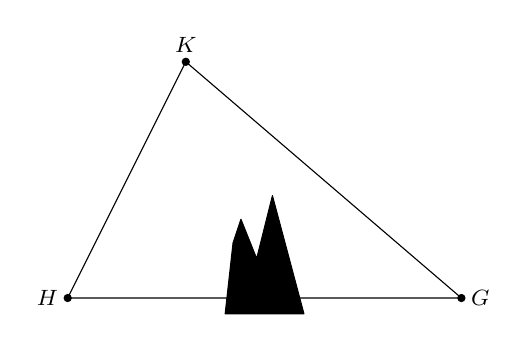
\begin{tikzpicture}[scale=1, font=\footnotesize, line join=round, line cap=round, >=stealth]
				\coordinate [label =left: $H$ ] (H) at (0,0);
				\coordinate [label =above: $K$ ] (K) at (1.5,3);
				\coordinate [label =right: $G$ ] (G) at (5,0);
				\draw (H)--(K)--(G)--cycle;	
				\draw[fill] (2,-0.2)--(2.1,0.7)--(2.2,1)--(2.4,0.5)--(2.6,1.3)--(3,-0.2)--cycle ;
				\foreach \diem in {H,K,G}\fill (\diem)circle(1.5pt);
			\end{tikzpicture}
		}
		\choice
		{\True $137025$ đồng}
		{ $107025$ đồng}
		{$12278$ đồng}
		{$137000$ đồng}	
		\loigiai{Tổng quãng đường mà ô tô phải đi là$ S = HK + KG = 15 + 20 = 35$ km.\\	
			Ô tô đi hết quãng đường tiêu thụ hết số lít xăng là 	$35 \cdot 0{,}3 = 10{,}5$ lít.\\	
			Ô tô đi từ H đến G hết số tiền xăng là
			$10{,}5 \cdot 13050 = 137025$ đồng.}
	\end{ex}	
	\begin{ex}%[Phạm Tuấn]%[0H2B3-1]
		Cho tam giác $ABC$ có góc $\widehat{B}=45^{\circ}$, $AC= 28$, $BC=25$. Tính số đo góc $A$  của tam giác (làm tròn kết quả đến hàng phần mười).
		\choice
		{$39{,}1^\circ$}
		{$40{,}2^\circ$}
		{\True $39{,}2^\circ$}
		{$40^\circ$}
		\loigiai{
			Áp dụng định lí sin ta có 
			\[ \dfrac{AC}{\sin B}=\dfrac{BC}{\sin A} \Rightarrow \sin A=\dfrac{BC\sin B}{AC}=\dfrac{25\sin 45^\circ}{28} =\dfrac{25\sqrt{2}}{56} \Rightarrow \widehat{A} \approx 39{,}2^\circ.\]
		}
	\end{ex}
	
	
	\begin{ex}%[Phạm Tuấn]%[0H2B3-1]
		Cho tam giác $ABC$ có góc $\widehat{B}=30^{\circ}, \widehat{C}=75^{\circ}$, $AB=20$. Độ dài cạnh $AC$ là
		\choice
		{$20(\sqrt{6}-\sqrt{2})$}
		{\True $10(\sqrt{6}-\sqrt{2})$}
		{$10(\sqrt{6}-1)$}
		{$5(\sqrt{6}+\sqrt{2})$}
		\loigiai{
			Áp dụng định lí sin ta có 
			\[ \dfrac{AC}{\sin B}=\dfrac{AB}{\sin C} \Rightarrow AC=\dfrac{AB\cdot\sin B}{\sin C}=\dfrac{20\cdot \sin 30^\circ}{\sin 75^\circ} =10(\sqrt{6}-\sqrt{2}).\]
		}
	\end{ex}
	
	\begin{ex}%[Phạm Tuấn]%[0H2B3-1] 
		Cho tam giác $ABC$ có $\widehat{B}= 30^\circ$, $\widehat{C}=45^\circ$ và $BC = 30\mathrm{~cm}$. Tính độ dài cạnh $AB$ (làm tròn kết quả đến hàng phần mười).
		\choice
		{$15 (\sqrt{3}+1) \mathrm{~cm}$}
		{$15 (\sqrt{3}-1) \mathrm{~cm}$}
		{$30 (2\sqrt{3}-1) \mathrm{~cm}$}
		{\True $30 (\sqrt{3}-1) \mathrm{~cm}$}
		\loigiai{
			Ta có $\widehat{A}= 180^\circ -  \widehat{B} -\widehat{C} = 180^\circ - 30^\circ-45^\circ  =105^\circ$. \\
			Áp dụng định lí sin ta có 
			\[
			\dfrac{AB}{\sin C} = \dfrac{BC}{\sin A} \Rightarrow AB = \dfrac{BC\sin C}{\sin A}  = \dfrac{30\sin 45^{\circ}}{\sin 105^{\circ}} = 30\sqrt{3}-30 \mathrm{~cm}.
			\]
		}
	\end{ex}
	
	
	\begin{ex}%[Phạm Tuấn]%[0H2B3-1]
		Cho tam giác $ABC$ có $BC= 11$, $\widehat{A} = 30^\circ$. Độ dài  cạnh $AB$ lớn nhất bằng bao nhiêu?
		\choice
		{$11\sqrt{3}$}
		{$\dfrac{22\sqrt{3}}{2}$}
		{\True $22$}
		{$11 (\sqrt{3}+1)$}
		\loigiai{
			Áp dụng định lí sin ta có 
			\begin{align*}
				\dfrac{AB}{\sin C} = \dfrac{BC}{\sin A} \Rightarrow AB = \dfrac{BC\sin C}{\sin A} = \dfrac{11 \sin C}{\sin 30^\circ}   \leq 22.
			\end{align*}
			Đẳng thức xảy ra khi $\widehat{C} = 90^\circ$. \\
			Vậy độ dài cạnh $AB$ lớn nhất bằng $22$.
		}
	\end{ex}
	
	\begin{ex}%[Phạm Tuấn]%[0H2B3-1] 
		Cho tam giác $ABC$ có $\widehat{C}= 30^\circ$ và $AB= 30 \mathrm{~cm}$. Tính bán kính đường tròn ngoại tiếp tam giác $ABC$.
		\choice
		{$30\sqrt{3} \mathrm{~cm}$}
		{$15 \sqrt{3}\mathrm{~cm}$}
		{\True $30 \mathrm{~cm}$}
		{$15 \mathrm{~cm}$}
		\loigiai{
			Áp dụng định lí sin ta có $R = \dfrac{AB}{2\sin C} = \dfrac{30}{2\sin 30^\circ} = 30 \mathrm{~cm}$. 
		}
	\end{ex}
	
	\begin{ex}%[Phạm Tuấn]%[0H2B3-1]
		Cho tam giác $MNK$ có $MN = a$, $MK=3a$, $\widehat{M} = 120^\circ$.  Tính bán kính đường tròn ngoại tiếp $R$ của tam giác $MNK$.
		\choice
		{\True $\dfrac{a\sqrt{39}}{3}$}
		{$\dfrac{a\sqrt{21}}{3}$}
		{$\dfrac{a\sqrt{33}}{3}$}
		{$\dfrac{a\sqrt{42}}{3}$}
		\loigiai{
			Áp dụng định lí côsin ta có
			\[
			NK^2= MN^2+MK^2-2MN \cdot MK \cos M = a^2+9a^2 -2 \cdot a \cdot 3a \cos 120^\circ = 13a^2 \Rightarrow NK=a\sqrt{13}.
			\]
			Áp dụng định lí sin ta có $R= \dfrac{NK}{2\sin M} = \dfrac{a\sqrt{13}}{2\sin 120^\circ} = \dfrac{a\sqrt{39}}{3}$.
		}
	\end{ex}
	
	
	\begin{ex}%[Phạm Tuấn]%[0H2B3-1] 
		\immini{
			Để đo bán kính của một chiếc đĩa cổ chỉ còn lại một phần, các nhà khảo cổ chọn $3$ điểm trên chiếc đĩa (hình vẽ). Biết $\widehat{A}=33^\circ$, $BC=15{,}3 \mathrm{~cm}$, tính bán kính của chiếc đĩa (làm tròn kết quả đến hàng phần mười).
			\choice
			{\True $13{,}8 \mathrm{cm}$}
			{$12{,}6 \mathrm{cm}$}
			{$12{,}9 \mathrm{cm}$}
			{$13{,}1 \mathrm{cm}$}
		}
		{
			\begin{tikzpicture}[scale=1, font=\footnotesize, line join=round, line cap=round,>=stealth]
				\coordinate (O) at (0,0); 
				\coordinate (A) at ($(O)+(131.4:3)$) ; 
				\coordinate (B) at ($(O)+(101.6:3)$) ; 
				\coordinate (C) at ($(O)+(41.7:3)$) ; 
				\coordinate (D) at ($(O)+(140:3)$) ; 
				\coordinate (E) at ($(O)+(90:1)$) ; 
				\coordinate (F) at ($(O)+(18:3)$) ; 
				\draw
				(D) 
				.. controls ++(0:0.5) and ++(150:0.5) .. (E)
				.. controls ++(180:-0.5) and ++(160: 0.5) .. (F)
				;
				\draw (A)--(B)--(C)--(A)  ; 
				\draw  (F) arc (18:140:3);
				\foreach \x/\g in {A/140,B/90,C/60} 
				\fill[black] (\x) circle (1.1pt)+(\g:3mm) node {$\x$};
			\end{tikzpicture}
		}
		\loigiai{
			Áp dụng định lí sin suy ra bán kính của chiếc đĩa là
			\[
			R = \dfrac{BC}{2\sin A} = \dfrac{15,3}{2\sin 33^\circ} \approx 13{,}8 \mathrm{~(cm)}. 
			\]
		}
	\end{ex}
	
	
	\begin{ex}%[Phạm Tuấn]%[0H2B3-2]
		Cho tam giác $ABC$ có $b^2= a^2+c^2+ac$. Khẳng định nào sau đây đúng?
		\choice
		{$\sin^2A = \sin^2B+ \sin^2C + \sin B\sin C$}
		{\True $\sin^2B = \sin^2A+ \sin^2C + \sin A\sin C$}
		{$\widehat{A} = 120^\circ$}
		{$\widehat{A} = 60^\circ$}
		\loigiai{
			Ta có
			\begin{align*}
				&b^2= a^2+c^2+ac \\
				\Leftrightarrow~& (2R\sin B)^2 =  (2R\sin A)^2+(2R\sin C)^2 + (2R\sin A) \cdot (2R\sin C )\\
				\Leftrightarrow~& \sin^2B = \sin^2A+ \sin^2C + \sin A\sin C. 
			\end{align*}
		}
	\end{ex}
	
	\begin{ex}%[Phạm Tuấn]%[0H2B3-2]
		Cho tam giác $ABC$. Khẳng định nào sau đây đúng?
		\choice
		{$\cot A = \dfrac{b^2+c^2-a^2}{2bc}$}
		{$\cot A = \dfrac{b^2+c^2-a^2}{abc}$}
		{$\cot A = \dfrac{R(b^2+c^2-a^2)}{2abc}$}
		{\True $\cot A = \dfrac{R(b^2+c^2-a^2)}{abc}$}
		\loigiai{
			Ta có
			\[
			\cot A = \dfrac{\cos A}{\sin A} = \dfrac{b^2+c^2 - a^2}{2bc \cdot \dfrac{a}{2R}} = \dfrac{R(b^2+c^2-a^2)}{abc}.
			\]
		}
	\end{ex}
	
	\begin{ex}%[Phạm Tuấn]%[0H2B3-1] 
		\immini{
			Cho tam giác $ABCD$ nội tiếp đường tròn tâm $O$.  Biết $\widehat{ACB} = 32^\circ$, $\widehat{ADC} = 75^\circ$ và $BC=8{,}8 \mathrm{~cm}$. Tính bán kính đường tròn đường tròn $(O)$. (Làm tròn kết quả đến hàng phần mười)
			\choice
			{$7{,}8 \mathrm{~cm}$}
			{$7{,}5 \mathrm{~cm}$}
			{$6{,}6 \mathrm{~cm}$}
			{\True $6{,}5 \mathrm{~cm}$}
		}
		{
			\begin{tikzpicture}[scale=1, font=\footnotesize, line join=round, line cap=round,>=stealth]
				\coordinate (O) at (1,1); 
				\coordinate (A) at ($(O)+(133:2.5)$) ; 
				\coordinate (B) at ($(O)+(198:2.5)$) ; 
				\coordinate (C) at ($(O)+(282:2.5)$) ; 
				\coordinate (D) at ($(O)+(0:2.5)$) ; 
				\draw (O) circle[radius=2.5cm];
				\draw (A)--(B)--(C)--(D)--(A)--(C) (B)--(D)  ; 
				\foreach \x/\g in {A/130,B/200,C/-90,D/0,O/-30} 
				\fill[black] (\x) circle (1.1pt)+(\g:3mm) node {$\x$};
			\end{tikzpicture}
		}
		\loigiai{
			Tứ giác $ABCD$ nội tiếp suy ra $\widehat{ADB} = \widehat{ACB} = 32^\circ $ $\Rightarrow \widehat{BCD} = \widehat{ADC} - \widehat{ADB} = 43^\circ$. \\
			Khi đó, bán kính đường tròn tâm $O$ là 
			\[
			R = \dfrac{BC}{2\sin \widehat{BDC}} = \dfrac{8{,}8}{2\sin 43^\circ} \approx 6{,}5 \mathrm{~(cm)}. 
			\]
		}
	\end{ex}
	\begin{ex}%[Phạm Tuấn]%[0H2B3-1]
		Cho tam giác $ABC$ có $AB=12$, $BC=15$, $AC=18$.  Tính $\widehat{A} + 2\widehat{C}$ (làm tròn kết quả đến hàng phần mười).
		\choice
		{$129{,}3^\circ$}
		{$142{,}7^\circ$}
		{$118{,}4^\circ$}
		{\True $138{,}6^\circ$}
		\loigiai{
			Áp dụng định lí côsin ta có
			\begin{align*}
				&\cos A = \dfrac{AB^2+AC^2-BC^2}{2 \cdot AB \cdot AC} = \dfrac{12^2+18^2-15^2}{2 \cdot 12 \cdot 18 } = \dfrac{9}{16} \Rightarrow \widehat{A} \approx  55{,}77^\circ. \\
				&\cos C = \dfrac{AC^2+BC^2-AB^2}{2 \cdot AC \cdot BC} = \dfrac{18^2+15^2-12^2}{2 \cdot 18 \cdot 15 } = \dfrac{3}{4} \Rightarrow \widehat{C} \approx  41{,}4^\circ.
			\end{align*}
			Suy ra $\widehat{A} + 2\widehat{C} \approx 138{,}6^\circ$. 
		}
	\end{ex}
	
	\begin{ex}%[Phạm Tuấn]%[0H2B3-1]
		Cho tam giác $ABC$ có góc $\widehat{A}=60^{\circ}$, $\widehat{B}=45^{\circ}$, $AB=25$. Độ dài cạnh $BC$ gần với giá trị nào nhất dưới đây?
		\choice
		{$22$}
		{\True $22{,}5$}
		{$24{,}5$}
		{$21{,}5$}
		\loigiai{
			Ta có $\widehat{C}=180^\circ - \widehat{A}-\widehat{B} =  180^\circ - 60^{\circ}-45^{\circ} = 75^{\circ}$. \\
			Áp dụng định lí sin ta có 
			\[ \dfrac{BC}{\sin A}=\dfrac{AB}{\sin C} \Rightarrow BC=\dfrac{AB\cdot\sin A}{\sin C}=\dfrac{25\cdot \sin 60^\circ}{\sin 75^\circ} \approx 22{,}4.\]
		}
	\end{ex}
	
	\begin{ex}%[Phạm Tuấn]%[0H2B3-1]
		Cho tam giác $ABC$ có $AB=8$, $AC = 11$, $\widehat{A}=30^\circ$.  Số đo góc $B$ gần với giá trị nào nhất dưới đây?
		\choice
		{$50{,}5^\circ$}
		{$45{,}8^\circ$}
		{$65{,}3^\circ$}
		{\True $55{,}2^\circ$}
		\loigiai{
			Áp dụng định lí côsin ta có 
			\[ BC^2=AB^2+AC^2-2AB \cdot AC \cos A =8^2+11^2-2 \cdot 8 \cdot 11 \cos 30^\circ \Rightarrow BC \approx 6{,}7.\]
			Áp dụng định lí sin ta có 
			\begin{align*}
				\dfrac{AC}{\sin B} = \dfrac{BC}{\sin A} \Rightarrow \sin B = \dfrac{AC\sin A}{BC}  = \dfrac{11 \sin 30^{\circ}}{6{,}7} \Rightarrow \widehat{B} \approx 55{,}2^\circ.  
			\end{align*}
		}
	\end{ex}

	\begin{ex}%[Phạm Tuấn]%[0H2B3-4] 
		\immini{
			Để đo bán kính của một chiếc đĩa cổ chỉ còn lại một phần, các nhà khảo cổ chọn ba điểm trên chiếc đĩa (hình vẽ).  Biết $AB=7{,}1 \mathrm{~cm}$, 
			$BC=16{,}3 \mathrm{~cm}$, $AC=19{,}6 \mathrm{~cm}$,  tính bán kính của chiếc đĩa (làm tròn kết quả đến hàng phần mười).
			\choice
			{$11{,}1 \mathrm{cm}$}
			{$9{,}8 \mathrm{cm}$}
			{\True $10{,}3 \mathrm{cm}$}
			{$10{,}1 \mathrm{cm}$}
		}
		{
			\begin{tikzpicture}[scale=1, font=\footnotesize, line join=round, line cap=round,>=stealth]
				\coordinate (O) at (0,0); 
				\coordinate (A) at ($(O)+(131.4:3)$) ; 
				\coordinate (B) at ($(O)+(101.6:3)$) ; 
				\coordinate (C) at ($(O)+(41.7:3)$) ; 
				\coordinate (D) at ($(O)+(140:3)$) ; 
				\coordinate (E) at ($(O)+(90:1)$) ; 
				\coordinate (F) at ($(O)+(18:3)$) ; 
				\draw
				(D) 
				.. controls ++(0:0.5) and ++(150:0.5) .. (E)
				.. controls ++(180:-0.5) and ++(160: 0.5) .. (F)
				;
				\draw (A)--(B)--(C)--(A)  ; 
				\draw  (F) arc (18:140:3);
				\foreach \x/\g in {A/140,B/90,C/60} 
				\fill[black] (\x) circle (1.1pt)+(\g:3mm) node {$\x$};
			\end{tikzpicture}
		}
		\loigiai{
			Áp dụng định lí côsin ta có
			\begin{align*}
				&BC^2=AB^2+AC^2-2AB \cdot AC \cos A  \\
				\Leftrightarrow~ & \cos A = \dfrac{AB^2+AC^2- BC^2}{2AB \cdot AC}  \\
				\Leftrightarrow~ & \cos A = \dfrac{7{,}1^2+19{,}6^2-16{,}3^2}{2 \cdot 7{,}1 \cdot 19{,}6}\\
				\Rightarrow~& \widehat{A} \approx 52{,}6427^\circ. 
			\end{align*}
			Áp dụng định lí sin suy ra bán kính của chiếc đĩa là
			\[
			R = \dfrac{BC}{2\sin A} = \dfrac{16{,}3}{2\sin 52{,}6427^\circ} \approx 10{,}3 \mathrm{~(cm)}. 
			\]
		}
	\end{ex}
	
	
	\begin{ex}%[Phạm Tuấn]%[0H2B3-4] 
		\immini{
			Để đo khoảng cách từ $A$ đến $B$ ngang qua một đầm lầy, người ta chọn điểm  $C$, sau đó khoảng cách từ $A$ đến $C$ và các góc $A$, $C$. Tính khoảng cách từ $A$ đến $B$ biết $AC=115\mathrm{~m}$, $\widehat{A}=98^\circ$, $\widehat{C}=52^\circ$.
			\choice
			{$188{,}1 \mathrm{~m}$}
			{$190{,}7 \mathrm{~m}$}
			{\True $181{,}2 \mathrm{~m}$}
			{$193{,}6 \mathrm{~m}$}
		}
		{
			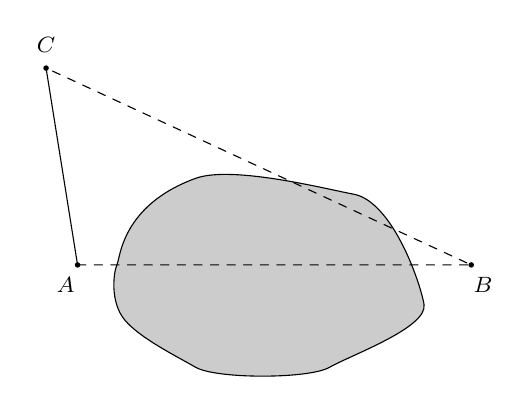
\begin{tikzpicture}[scale=1, font=\footnotesize, line join=round, line cap=round,>=stealth]
				\path
				(2,2) coordinate (A)
				(7,2) coordinate (B)
				(1.6,4.5) coordinate (C)
				(2.5,2) coordinate (D)
				(3.5,3.1) coordinate (E)
				(5.5,2.9) coordinate (F)
				(6.4,1.5) coordinate (G)
				(5.2,0.7) coordinate (H)
				(3.5,0.7) coordinate (I)
				(2.6,1.3) coordinate (J)
				;
				\draw[fill=gray!40] 
				(D) 
				.. controls ++(65:0.1) and ++(200: 1) .. (E)
				.. controls ++(200:-0.5) and ++(170: 0.3) .. (F)
				.. controls ++(170:-0.5) and ++(100: 0.3) .. (G)
				.. controls ++(100:-0.3) and ++(30: 0.3) .. (H)
				.. controls ++(30:-0.3) and ++(150: -0.3) .. (I)
				.. controls ++(150:0.3) and ++(130: -0.3) .. (J)
				.. controls ++(130:0.3) and ++(65: -0.1) .. (D)
				;
				\draw[dashed] (A)--(B)--(C) ;
				\draw (A)--(C)   ;
				\foreach \x/\g in {A/-120,B/-60,C/90} 
				\fill[black] (\x) circle (1pt)+(\g:3mm) node {$\x$};
			\end{tikzpicture}
		}
		\loigiai{
			Ta có $\widehat{B} = 180^\circ -  \widehat{A} -\widehat{C}  = 30^\circ $. \\
			Áp dụng định lí sin ta có 
			\begin{align*}
				\dfrac{AB}{\sin C} = \dfrac{AC}{\sin B} \Rightarrow AB = \dfrac{AC\sin C}{\sin B} = \dfrac{115 \sin 52^\circ}{\sin 30^\circ} \approx 181{,}2 \mathrm{~(m).}
			\end{align*}
		}
	\end{ex}
	
	\begin{ex}%[Phạm Tuấn]%[0H2K3-1] 
		\immini{
			Cho tam giác $A B C$ có $AB=8$, $AC=10$, $\widehat{A}=75^{\circ}$. $M$ là điểm thuộc cạnh $BC$  sao cho $CM=2BM$. Bán kính đường tròn ngoại tiếp tam giác  $ABM$  gần nhất với giá trị nào dưới đây?
			\choice
			{$3{,}8$}
			{\True $4{,}1$}
			{$3{,}6$}
			{$3{,}5$}
		}
		{
			\begin{tikzpicture}[scale=1, font=\footnotesize, line join=round, line cap=round,>=stealth]
				\path
				(0,0) coordinate (B)
				(4,0) coordinate (C)
				;
				\coordinate (M) at ($(B)!{1/3}!(C)$) ;
				\coordinate (A) at ($(B)+(66:3.5)$) ; 
				\draw (A)--(B)--(C)--(A) (A)--(M) ;
				\foreach \x/\g in {A/90,B/-120,C/-60,M/-90} 
				\fill[black] (\x) circle (1pt)+(\g:3mm) node {$\x$};
			\end{tikzpicture}
		}
		\loigiai{
			Áp dụng định lí côsin ta có 
			\begin{align*}
				&BC^2=AB^2+AC^2-2AB \cdot AC \cos A =8^2+10^2-2 \cdot 8 \cdot 10 \cos 75^\circ  \Rightarrow BC\approx  11{,}072; \\
				& \cos B = \dfrac{AB^2+BC^2-AC^2}{2AB \cdot BC} \approx  0{,}4888 \Rightarrow \widehat{B} \approx  60{,}4^\circ.
			\end{align*}
			Ta có $CM=2BM \Rightarrow BM = \dfrac{1}{3}BC =  3{,}69$. \\
			Áp dụng định lí côsin ta có 
			\begin{align*}
				AM^2=AB^2+BM^2-2AB \cdot BM \cos B =8^2+3{,}69^2-2 \cdot 8 \cdot 3{,}69 \cdot  0{,}4888 \Rightarrow AM \approx 6{,}983.
			\end{align*}
			Áp đụng định lí sin,  suy ra bán kính đường tròn ngoại tiếp tam giác $ABM$ là
			\[
			R = \dfrac{AM}{2\sin B} = \dfrac{6{,}983}{2\sin 60{,}4^\circ} \approx 4. 
			\]
		}
	\end{ex}
	
	\begin{ex}%[Phạm Tuấn]%[0H2B3-4] 
		\immini{
			Tàu $A$ rời cảng vào lúc 6h00 và chuyển động với vận tốc $30\mathrm{~km/h}$.  Tàu $B$ rời cảng vào lúc 6h30. Vào lúc 9h30 tàu $B$ gặp tàu $A$ tại điểm $C$ (hình vẽ). Giả sử hai tàu chuyển động thẳng và có vận tốc không đổi trong suốt quá trình di chuyển, tính vận tốc tàu $B$ (kết quả làm tròn đến hàng phần mười).
			\choice
			{$42{,}5\mathrm{~km/h}$}
			{\True $44{,}8\mathrm{~km/h}$}
			{$41{,}7\mathrm{~km/h}$}
			{$45{,}4\mathrm{~km/h}$}
		}
		{
			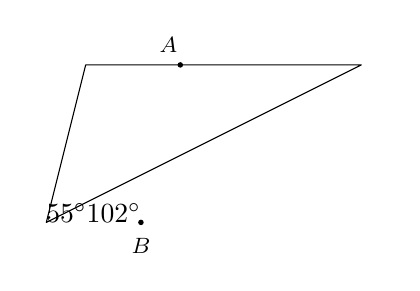
\begin{tikzpicture}[scale=1, font=\footnotesize, line join=round, line cap=round,>=stealth]
				\path
				(0.5,2) coordinate (A)
				(0,0) coordinate (B)
				(4,2) coordinate (C)
				;
				\draw (A)--(B)--(C)--(A) ;
				
				\tkzMarkAngle[arc=ll, size=0.5,mark=0](C,B,A)
				\tkzLabelAngle[pos=0.9](C,B,A) {$55^{\circ}$}
				\tkzMarkAngle[arc=ll, size=0.5,mark=0](B,A,C)
				\tkzLabelAngle[pos=0.9](B,A,C) {$102^{\circ}$}
				\foreach \x/\g in {A/120,B/-90,C/60} 
				\fill[black] (\x) circle (1pt)+(\g:3mm) node {$\x$};
			\end{tikzpicture}
		}
		\loigiai{
			Khoảng cách từ $A$ đến $C$ là $30 \cdot 2{,}5 =75 \mathrm{~km}$. \\
			Áp dụng định lí sin ta có 
			\begin{align*}
				\dfrac{AC}{\sin B} = \dfrac{BC}{\sin A} \Rightarrow BC = \dfrac{AC\sin A}{\sin B}  = \dfrac{75 \sin 102^{\circ}}{\sin 55^{\circ}}.
			\end{align*}
			Suy ra vận tốc của tàu $B$ là  $v= \dfrac{BC}{2} = \dfrac{75 \sin 102^{\circ}}{2\sin 55^{\circ}}  \approx 44{,}8\mathrm{~km/h}$.
		}
	\end{ex}

	\begin{ex}%[0H2Y3-1]
		Chọn công thức đúng trong các đáp án sau
		\choice
		{$S=\dfrac{1}{2}bc\sin B$}
		{\True $S=\dfrac{1}{2}bc\sin A$}
		{$S=\dfrac{1}{2}ab\sin B$}
		{$S=\dfrac{1}{2}ac\sin A$}
		\loigiai{
			Công thức đúng là $S=\dfrac{1}{2}bc\sin A$.
		}
	\end{ex}
	\begin{ex}%[0H2B3-2]
		Cho $\triangle ABC$ với các cạnh $AB=c$, $AC=b$, $BC=a$. Gọi $R$, $r$, $S$ lần lượt là bán kính đường tròn ngoại tiếp, nội tiếp và diện tích của tam giác $ABC$. Trong các phát biểu sau, phát biểu nào \textbf{sai}?
		\choice
		{$S=\dfrac{abc}{4R}$}
		{\True $R=\dfrac{a}{\sin A}$}
		{$S=\dfrac{1}{2}ab\sin C$}
		{$a^2+b^2-c^2=2ab\cos C$}
		\loigiai{Theo định lý Sin trong tam giác, ta có $\dfrac{a}{\sin A}=2R$. Nên mệnh đề \textbf{sai} là ``$R=\dfrac{a}{\sin A}$''.}
	\end{ex}
	
	\begin{ex}%[0H2Y3-1]
		Cho tam giác $ABC$ có $AB=4$, $AC=3$, $\widehat{BAC}=30^\circ$. Khi đó diện tích tam giác $ABC$ bằng
		\choice
		{\True $3$}
		{$4\sqrt{3}$}
		{$6\sqrt{3}$}
		{$6$}
		\loigiai{
			Ta có $S_{ABC}=\dfrac{1}{2}AB\cdot AC\cdot\sin\widehat{BAC}=\dfrac{4\cdot 3\cdot\sin30^\circ}{2}=3$.
		}
	\end{ex}
	\begin{ex}%[0H2B3-1]
		Tìm chu vi tam giác $ABC$, biết $AB=6$ và $2\sin A=3\sin B=4\sin C$.
		\choice
		{\True $26$}
		{$13$}
		{$5\sqrt{26}$}
		{$10\sqrt{6}$}
		\loigiai{
			Từ $2\sin A=3\sin B=4\sin C$ suy ra $2BC=3AC=4AB$.\\
			Mà $AB=6$ nên $AC=8$, $BC=12$. Chu vi tam giác bằng $26$.
		}
	\end{ex}
	\begin{ex}%[0H2B3-1]
		Cho tam giác $ABC$ có $a=13$ m, $b= 14$ m, $c=15$ m. Tính diện tích $S$ của tam giác $ABC$.
		\choice
		{\True $S= 84$ m$^2$}
		{$S= 90$ m$^2$}
		{$S= 76$ m$^2$}
		{$S= 80$ m$^2$}
		\loigiai{
			Ta có $p=\dfrac{a+b+c}{2} =21$ và $S=\sqrt{p(p-a)(p-b)(p-c)}=\sqrt{21(21-13)(21-14)(21-15)} =84$ m$^2$.	
		}
	\end{ex}
	\begin{ex}%[0H2B3-1]
		Cho tam giác $ABC$. Biết $AB=3$, $AC=4$, $BC>5$ và diện tích tam giác $ABC$ bằng $3\sqrt{3}$. Số đo góc $\widehat{BAC}$ bằng
		\choice
		{\True $120^{\circ}$}
		{$60^{\circ}$}
		{$135^{\circ}$}
		{$45^{\circ}$}
		\loigiai{
			Ta có $S_{\triangle ABC}=\dfrac{1}{2}\cdot AB \cdot AC \cdot \sin{\widehat{BAC}}$, suy ra 
			\[\sin{\widehat{BAC}}=\dfrac{2S_{\triangle ABC}}{AB \cdot AC}=\dfrac{2\cdot 3\sqrt{3}}{3 \cdot 4}=\dfrac{\sqrt{3}}{2} \Rightarrow \hoac{&\widehat{BAC}=60^\circ\\&\widehat{BAC}=120^\circ}.\]
			Mặt khác, ta có $\cos{\widehat{BAC}}=\dfrac{AB^2+AC^2-BC^2}{2\cdot AB \cdot AC}<\dfrac{9+16-25}{2 \cdot 3 \cdot 4}=0$.\\
			Vậy $\widehat{BAC}=120^{\circ}$.
		}
	\end{ex}
	\begin{ex}%[0H2K3-1]
		Cho tam giác $ABC$ có $AB=2$, $AC=3$, $BC=4$. Khi đó độ dài đường cao của tam giác $ABC$ kẻ từ $A$ bằng
		\choice
		{$\dfrac{3\sqrt{15}}{2}$}
		{$\dfrac{3\sqrt{15}}{4}$}
		{\True $\dfrac{3\sqrt{15}}{8}$}
		{$3\sqrt{15}$}
		\loigiai{
			Ta có nữa chu vi $p=\dfrac{2+3+4}{2}=\dfrac{9}{2}$.\\
			Suy ra $S_{ABC}=\sqrt{p(p-AB)(p-AC)(p-BC)}=\sqrt{\dfrac{9}{2}\left(\dfrac{9}{2}-2\right)\left(\dfrac{9}{2}-3\right)\left(\dfrac{9}{2}-4\right)}=\dfrac{3\sqrt{15}}{4}$.\\
			Suy ra độ dài đường cao kẻ từ $A$ bằng $\dfrac{2S_{ABC}}{BC}=\dfrac{2\cdot\dfrac{3\sqrt{15}}{4}}{4}=\dfrac{3\sqrt{15}}{8}$.
		}
	\end{ex}
	\begin{ex}%[0H2B3-1]
		Cho tam giác $ABC$ có $AB=9$cm, $AC=12$cm và $BC=15$cm. Khi đó đường trung tuyến $BM$ của tam giác $ABC$ có độ dài là 
		\choice
		{$117$cm}
		{$18{,}82$cm}
		{$10{,}82$cm}
		{\True $7{,}5$cm}
		\loigiai{
			Ta có $m_a^2= \dfrac{2(b^2+c^2)-a^2}{4}=\dfrac{2(12^2+9^2)-15^2}{4}= \dfrac{225}{4} \Rightarrow m_a= 7{,}5$. 		
		}
	\end{ex}
	\begin{ex}%[0H2K3-1]
		Tam giác $ABC$ có các trung tuyến $m_a=10$, $m_b=8$ và $m_c=6$. Tính diện tích $S$ của tam giác $ABC$.
		\choice
		{\True $S=32$}
		{$S=24$}
		{$S=48$}
		{$S=64$}
		\loigiai{
			\immini{
				Gọi $M,N,P$ lần lượt là trung điểm $BC,CA,AB$, $G$ là trọng tâm tam giác $ABC$.\\
				Theo bài ra ta có $AM=10,BN=8,CP=6$.\\
				Lấy $Q$ đối xứng với $G$ qua $M$ thì $BGCQ$ là hình bình hành và ta có $BQ=CG=\dfrac{2CP}{3}=4$, $QG=2GM=\dfrac{2AM}{3}=\dfrac{20}{3}$.\\
				Mà $BG=\dfrac{2BN}{3}=\dfrac{16}{3}$ nên $QG^2=BG^2+BQ^2$ hay $\triangle BGQ$ vuông tại $B$.\\
				Suy ra $S_{BGQ}=\dfrac{BG\cdot BQ}{2}=\dfrac{32}{3}$.\\
				Mà $S_{BGQ}=S_{BGC}=\dfrac{1}{3}S_{ABC}\Rightarrow S_{ABC}=32$.
			}{
				\begin{tikzpicture}[scale=1, font=\footnotesize, line join=round, line cap=round,>=stealth]
					\tkzInit[xmin=-0.5, xmax=5.5, ymin=-0.5, ymax=6.5]
					\tkzClip
					\tkzDefPoints{4/1.5/C,2/0/Q}
					\tkzDefPointBy[rotation=center C angle -90](Q)\tkzGetPoint{g}
					\tkzDefPointBy[homothety=center C ratio 3/4](g)\tkzGetPoint{G}
					\tkzDefPointBy[symmetry=center G](Q)\tkzGetPoint{A}
					\tkzDefMidPoint(G,Q)\tkzGetPoint{M}
					\tkzDefPointBy[symmetry=center M](C)\tkzGetPoint{B}
					\tkzDefMidPoint(A,B)\tkzGetPoint{P}
					\tkzDefMidPoint(A,C)\tkzGetPoint{N}
					\tkzDrawPoints[fill=black](C,G,Q,B,A,P,M,N)
					\tkzDrawSegments(A,B B,C C,A A,Q B,N C,P B,Q C,Q)
					\tkzLabelPoints[above](A)
					\tkzLabelPoints[below](B,Q,C)
					\tkzLabelPoints[right](G,N)
					\tkzLabelPoints[below right](M)
					\tkzLabelPoints[left](P)
				\end{tikzpicture}
			}
		}
	\end{ex}
	\begin{ex}%[0H2K3-4]
		Cho tam giác $ABC$ có chu vi bằng $26$ cm và $\dfrac{\sin A}{2} = \dfrac{\sin B}{6} = \dfrac{\sin C}{5}$. Tính diện tích của tam giác $ABC$. 
		\choice
		{$ 2\sqrt{23} $ (cm$^2$)}
		{$ 6\sqrt{13} $ (cm$^2$)}
		{\True $ 3\sqrt{39} $ (cm$^2$)}
		{$ 5\sqrt{21} $ (cm$^2$)}
		\loigiai{
			Ta có $\dfrac{\sin A}{2} = \dfrac{\sin B}{6} = \dfrac{\sin C}{5} \Leftrightarrow \heva{&\sin B = 3\sin A\\&\sin C = \dfrac{5}{2}\sin A.}$\\
			Mặt khác theo định lí $\sin$ trong tam giác $ABC$ ta có
			$\dfrac{a}{\sin A} = \dfrac{B}{\sin B} = \dfrac{c}{\sin C} \Leftrightarrow \heva{&b = 3a\\&c = \dfrac{5}{2}a.}$\\
			Mà $a + b + c = 26 \Leftrightarrow a + 3a + \dfrac{5}{2}a = 26 \Leftrightarrow \dfrac{13a}{2} = 26 \Leftrightarrow a = 4 \Rightarrow b = 12$ và $c = 10$.\\
			Vậy diện tích tam giác $ABC$ là 
			$$S_{\triangle ABC} = \sqrt{13(13 - 4)(13 - 12)(13 - 10)} = 3\sqrt{39} \,\, (\textrm{cm}^2).$$
		}
	\end{ex}
	\begin{ex}%[0H2B3-1]
		Cho tam giác $ABC$ vuông tại $C$ và $BC=6$, $CA=8$. Tính bán kính đường tròn nội tiếp của tam giác $ABC$.
		\choice
		{\True $2$}
		{$2\sqrt{2}$}
		{$\sqrt{2}$}
		{$4$}
		\loigiai{
			Vì tam giác $ABC$ vuông tại $C$ nên $AB=\sqrt{AC^2+BC^2}=10$ và $S_{ABC}=\dfrac{1}{2}\cdot AC\cdot BC=24$.\\
			Mặt khác $p=\dfrac{6+8+10}{2}=12$, $S_{ABC}=p\cdot r\Rightarrow r=\dfrac{S_{ABC}}{p}=\dfrac{24}{12}=2$.
		}
	\end{ex}
	
	\begin{ex}%[0H2T3-4]
		Từ vị trí $A$ người ta quan sát một cây cao (Hình vẽ). Biết $AH=4$ m, $HB=20$ m, $\widehat{BAC}=45^{\circ}$. Chiều cao của cây gần nhất với giá trị nào sau đây?
		\begin{center}
			\usetikzlibrary{decorations.pathmorphing,shapes}
			\tikzset{
				treetop/.style = {
					decoration={random steps, segment length=0.4mm},
					decorate
				},
				trunk/.style = {
					decoration={random steps, segment length=2mm, amplitude=0.2mm},
					decorate
				}
			}
			\tikzset{
				man/.pic={%
					\fill [rounded corners=1.5] (0,0.4) -- (0,0.4) -- (0.4,0.5) -- (0.4,0.4) --
					(0.325,0.4) -- (0.325,0.7) -- (0.3,0.7) -- (0.3,0) -- (0.225,0) --
					(0.225,0.4) -- (0.175,0.4) -- (0.175,0) -- (0.1,0) -- (0.1,0.7) --
					(0.075,0.7) -- (0.075,0.4) -- cycle;
					\fill (0.2,0.9) circle (0.1);
					\coordinate (-head) at (0.2,1);
					\coordinate (-foot) at (0.2,0);
				}
			}
			\begin{tikzpicture}
				\path 
				(-5,-2.09) coordinate (A)
				(0,1.5) coordinate (C)
				(0.1,-3) coordinate (T)
				(-5,-3) coordinate (H)
				(0,-3) coordinate (B)		
				;
				%\pic[red] at (-6.3,-3) (myman) {man};
				\foreach \w/\f in {0.3/30,0.2/50,0.1/70} {
					\fill [brown!\f!black, trunk] (0,0) ++(-\w/2,0) rectangle +(\w,-3);
				}
				\foreach \n/\f in {1.4/40,1.2/50,1/60,0.8/70,0.6/80,0.4/90} {
					\fill [green!\f!black, treetop] ellipse (\n/1.5 and \n);
				}
				\draw (H)--(T) (A)--(H) (A)--(C) (A)--(B);
				\pic[draw,"$45^{\circ}$", angle eccentricity=1.4,angle radius=0.8cm]{angle=B--A--C};
				\pic[draw,"$ $", angle eccentricity=1.4,angle radius=0.7cm]{angle=B--A--C};
				\draw pic[draw, angle radius=2mm]{right angle=B--H--A};
				\path (H)--(B) node[below,midway,sloped]{$20$ m};
				\foreach \x/\g in {A/180,B/-90,C/90,H/-90} \fill[black] (\x)+(\g:.3) node {$\x$};
			\end{tikzpicture}
		\end{center}
		\choice
		{$14$ m}
		{$15$ m}
		{\True $17$ m}
		{$16$ m}
		\loigiai{\immini{Ta có $AB= \sqrt{AH^2 + BH^2} = \sqrt{4^2+20^2} = 4 \sqrt{26}$.\\
				$\tan \widehat{HAB} = \dfrac{HB}{HA} = \dfrac{20}{4} = 5 \Rightarrow \widehat{HAB} \approx 78{,}69^{\circ}$.\\
				Do $AH \parallel BC$ nên $ \widehat{ABC} = \widehat{HAB} \approx 78{,}69^{\circ}$.\\
				$\widehat{ACB} = 180^{\circ} - 45^{\circ} - \widehat{ABC} \approx 56{,}31^{\circ}$.\\
				Áp dụng định lí hàm số $\sin$ trong tam giác $ABC$ ta có
				$$ \dfrac{BC}{\sin 45^{\circ}} = \dfrac{AB}{\sin 56{,}31^{\circ}} = \dfrac{4 \sqrt{26}}{\sin 56{,}31^{\circ}} \Rightarrow BC \approx  17{,}33.$$	}
			{\begin{tikzpicture}[scale=0.8, font=\footnotesize,line join = round, line cap = round, >=stealth]
					\tkzDefPoints{-5/-2.09/A, 0/1.5/C, 0.1/-3/T, -5/-3/H,0/-3/B}
					\tkzDrawSegments(H,B A,H A,C A,B B,C)
					\tkzMarkAngles[size=0.6,arc=ll](B,A,C)
					\tkzMarkRightAngles(B,H,A)
					\tkzLabelAngles[pos=1.1](B,A,C){$45^{\circ}$}
					\tkzLabelPoints[above](C)
					\tkzLabelPoints[above](A)
					\tkzLabelPoints[below](B)
					\tkzLabelPoints[below](H)
			\end{tikzpicture}}
		}
	\end{ex}
	
	\begin{ex}%[0H2G3-1]
		Một miếng giấy hình tam giác $ABC$ diện tích $S$ có $I$ là trung điểm $BC$ và $O$ là trung điểm của $AI$. Cắt miếng giấy theo một đường thẳng qua $O$, đường thẳng này đi qua $M$, $N$ lần lượt trên các cạnh $AB$, $AC$. Khi đó diện tích miếng giấy chứa điểm $A$ có diện tích thuộc đoạn $\left[mS; nS\right]$. Tính $T = \dfrac{1}{m} + \dfrac{1}{n}$.
		\choice
		{$T = \dfrac{7}{12}$}
		{$T = 12$}
		{\True $T = 7$}
		{$T=\dfrac{12}{7}$}
		\loigiai
		{\immini
			{Ta có $\dfrac{S_{\triangle AMN}}{S_{\triangle ABC}} = \dfrac{AM}{AB}\cdot\dfrac{AN}{AC}$\\
				Dễ thấy $S_{\triangle ABI} = S_{\triangle ACI} = \dfrac{1}{2}\cdot S_{\triangle ABC}$.\\
				Mặt khác   
				\begin{eqnarray*}
					&{  }&\dfrac{S_{\triangle AMO}}{S_{\triangle ABI}} = \dfrac{AO}{AI}\cdot\dfrac{AM}{AB}\\
					&=& \dfrac{1}{2}\cdot\dfrac{AM}{AB}\Rightarrow \dfrac{2\cdot S_{\triangle AMO}}{S_{\triangle ABC}} = \dfrac{1}{2}\cdot\dfrac{AM}{AB}\quad (1)
				\end{eqnarray*}	
			}
			{\begin{tikzpicture}[scale=1, font=\footnotesize, line join=round, line cap=round, >=stealth]
					\clip(-1,-1) rectangle (6.5,4.5);
					\tkzDefPoints{0/0/B,1/4/A, 6/0/C}
					\tkzDefMidPoint(B,C) \tkzGetPoint{I}
					\tkzDefMidPoint(A,I) \tkzGetPoint{O}
					\tkzDefBarycentricPoint(A=2,B=3)
					\tkzGetPoint{M}
					\tkzInterLL(M,O)(A,C)\tkzGetPoint{N}
					\tkzInterLL(B,O)(A,C)\tkzGetPoint{N'}
					\tkzInterLL(C,O)(A,B)\tkzGetPoint{M'}
					\tkzDefLine[parallel = through I](B,N') \tkzGetPoint{c}
					\tkzInterLL(I,c)(A,C)\tkzGetPoint{I'}
					\tkzLabelPoints[above](A)
					\tkzLabelPoints[left](M,M')
					\tkzLabelPoints[above right](N,N',I')
					\tkzLabelPoints[below left](I)
					\tkzLabelPoints[below](B,C)
					\tkzDrawPoints[fill=black](A,B,C,M,N,O,I,M',N',I')
					\tkzDrawSegments(A,B B,C C,A A,I M,N)
					\tkzDrawSegments [dashed](B,N' C,M' I,I')
					\draw ($(O)+(-0.1,-0.35)$) node {$O$};
				\end{tikzpicture}
			}\noindent
			Tương tự  $\dfrac{2\cdot S_{\triangle ANO}}{S_{\triangle ABC}} = \dfrac{1}{2}\cdot\dfrac{AN}{AC}\quad (2)$.	
			Từ $(1)$ và $(2)$ suy ra 
			$$\dfrac{2\cdot S_{\triangle AMN}}{S_{\triangle ABC}} = \dfrac{1}{2}\cdot\left(\dfrac{AM}{AB} + \dfrac{AN}{AC}\right)\Leftrightarrow \dfrac{S_{\triangle AMN}}{S_{\triangle ABC}} = \dfrac{1}{4}\cdot\left(\dfrac{AM}{AB} + \dfrac{AN}{AC}\right)$$
			Theo bất đẳng thức Côsi suy ra 
			$$\dfrac{AM}{AB} + \dfrac{AN}{AC}\geq 2\sqrt{\dfrac{AM}{AB}\cdot \dfrac{AN}{AC}}\Leftrightarrow \left(\dfrac{AM}{AB} + \dfrac{AN}{AC}\right)^2\geq 4\cdot \dfrac{AM}{AB}\cdot \dfrac{AN}{AC}$$
			Đặt $t = \dfrac{S_{\triangle AMN}}{S_{\triangle ABC}}$ điều kiện $t > 0$. Khi đó ta có  $16t^2\geq 4t\Leftrightarrow t\geq\dfrac{1}{4}$ suy ra $S_{\triangle AMN}\geq \dfrac{1}{4}\cdot S_{ABC}$.\\
			Khi $M\equiv B$ suy ra $N\equiv N'$ khi đó $S_{\triangle AMN} =  S_{\triangle ABN'}$.\\
			Mà $S_{\triangle ABN'} = S_{\triangle ABO}+ S_{\triangle AON'}$.\\
			Dễ thấy $S_{\triangle ABO} = \dfrac{1}{2}\cdot S_{\triangle ABI} = \dfrac{1}{4}\cdot S_{\triangle ABC}$.\\
			Mặt khác từ $I$ kẻ $II'\parallel BN'$, khi đó $AN' = N'I' = I'C$ nên
			$$\dfrac{S_{\triangle AON'}}{S_{\triangle AIC}} = \dfrac{AO}{AI}\cdot\dfrac{AN'}{AC} = \dfrac{1}{2}\cdot\dfrac{1}{3} = \dfrac{1}{6}\Rrightarrow S_{\triangle AON'} = \dfrac{1}{6}\cdot S_{\triangle AIC}$$
			Do đó $S_{\triangle AON'} = \dfrac{1}{12}\cdot S_{\triangle ABC}$ nên $S_{\triangle ABN'} = \dfrac{1}{4}\cdot S_{\triangle ABC} + \dfrac{1}{12}\cdot S_{\triangle ABC} = \dfrac{1}{3}\cdot S_{\triangle ABC}$.\\
			Khi $N\equiv C$ suy ra $M\equiv M'$ khi đó $S_{\triangle AMN} =  S_{\triangle ACM'}$.\\
			Chứng minh tương tự, ta có  $S_{\triangle ACM'} = \dfrac{1}{3}\cdot S_{\triangle ABC}$.\\
			Do đó khi $MN$ đi thay đổi qua $O$ suy ra 
			$$\dfrac{1}{4}\cdot S_{\triangle ABC}\leq  S_{\triangle AMN}\leq  \dfrac{1}{3}\cdot S_{\triangle ABC}\Leftrightarrow \dfrac{1}{4}\cdot S\leq S_{\triangle AMN} \leq  \dfrac{1}{3}\cdot S$$
			Do đó $m = \dfrac{1}{4}$ và $n = \dfrac{1}{3}$ nên $T = \dfrac{1}{m} + \dfrac{1}{n} = 4 + 3 = 7$.
		}
	\end{ex}
	\Closesolutionfile{ans}
	\Closesolutionfile{ansbook}
	% % \indapan{10}{ans/ans-0D3-6-TN}
	